\documentclass{sice-si}

% タイトルと著者名
\title{視覚と行動のend-to-end学習により経路追従行動を\\
オンラインで模倣する手法の提案\\
-トポロジカルマップとシナリオに基づく経路選択機能の追加と検討-\\} % 和文タイトル
\name{○春山健太(千葉工大),藤原柾(千葉工大)馬場琉生(千葉工大)\\石黒巧(千葉工大)
上田隆一(千葉工大)林原靖男(千葉工大)} % 著者名
\etitle{A proposal for an online imitation method of
path-tracking behavior by end-to-end learning of vision and action\\
- Adding and consideration  of path selection function \\based on a topological map and scenario -} % 英文タイトル
\ename{○Kenta HARUYAMA (CIT),Masaki FUJIWARA (CIT),Ryusei BABA (CIT),\\
Takumi ISHIGURO (CIT),Ryuichi UEDA (CIT),Yasuo HAYASHIBARA (CIT)}	%著者名(英)

\begin{document}
% アブストラクト
\abst{
We proposed an online imitation of path-following behavior based on end-to-end learning of vision and behavior. In this study, the robot moves autonomously to the destination based on camera images and target directions.
In this paper, we add a method to generate target directions from camera images.
We introduce a method for autonomous movement to a destination based on camera images without requiring a metric map.
Experiments using a real robot verify the effectiveness of the proposed method.
}

% タイトルの出力
\maketitle

% 本文
\section{緒言}
本研究グループでは,LiDARなどをセンサ入力とする行動を
カメラ画像を入力とする行動へ模倣することで,
ロボットに複数のナビゲーション手段を与える手法を提案してきた
\cite{haruyama2022}\cite{fujiwara2023}.
% 2つのナビゲーション手段が得られる.この2つの手段を状況
% に応じて高い信頼性が見込まれる方を選択することで,
% 経路追従を継続できる可能性が高まる.
% end-to-end学習により,カメラ画像と目標とする
% を
% 入力として,経路を追従する行動をオンラインで模倣する手法を提案し,
% 実験により手法の有効性を検証してきた
これまで提案した手法では,
LiDARやオドメトリ,事前に作成したメトリックマップを入力とする
地図に基づいたルールベース制御器によって
経路追従する.ここでいう地図に基づいたルールベース制御器は
ROS Navigation Stack\cite{ros-navigation}である
その際,この行動をカメラ画像と進行方向の情報(以後,目標方向と呼ぶ)を
入力としてオンラインで模倣するように学習する.
これにより,Fig.\ref{fig:camera_base}に示すカメラ画像と
前述のルールベース制御器から生成される目標方向に基づき,
経路を選択して追従する行動を獲得できる.
\par
前報\cite{haruyama2022}\cite{fujiwara2023}ではFig.\ref{fig:camera_base}のように
カメラ画像から目標方向を生成していなかった.
そこで,カメラ画像に基づいて目標方向を生成する方法を検討する.
本稿では,カメラ画像から目標方向を生成する方法として,
島田ら\cite{shimada2020}が提案したトポロジカルマップと「条件」や「行動」による経路の表現
(以後,シナリオと呼ぶ)をこれまで提案した手法へ追加する.
そして,カメラ画像とトポロジカルマップから生成されるシナリオに基づいて,
目的地まで自律移動する手法を新たに提案する.
この手法により,事前に作成したメトリックマップを必要せずに,
カメラ画像を入力として目的地まで自律移動できる可能性がある.
\par
メトリックマップを用いず,カメラ画像に基づいて自律移動を行う研究はいくつかある.
Dhruvら\cite{shah2022lmnav}は大規模な事前学習モデルを用いて,自然言語による指示から,
画像によるナビゲーションをend-to-endで行う手法を提案している.
またmiyamotoら\cite{seg_meizi}はカメラ画像と深層学習による走行可能領域の検出と
トポロジカルマップを用いたナビゲーション手法を提案している.
これらの手法では,補助的ではあるが,Global Navigation Satellite System(GNSS)
やホイールオドメトリといった情報を
必要とすることが本稿で提案する手法との違いに挙げられる.
本稿では,提案手法の有効性を実ロボットを用いた実験により検証することを目的とする.
\par
% 本稿では,カメラ画像を入力とする経路追従に対して,
% 島田らが提案した「突き当りまで」という「条件」や「直進」などの「行動」
% で表現されるシナリオ\cite{shimada2020}を
% 事前に作成したメトリックマップを用いず,
% トポロジカルマップとそこから生成されるシナリオを用いてとカメラ画像と
% 基づいてメトリックマップなしで目的地まで自律移動する手法を提案する.
% また,実ロボットを用いた実験を通して,提案した手法の有効性を検証する.
% \begin{figure}[htb
%     \centering
%      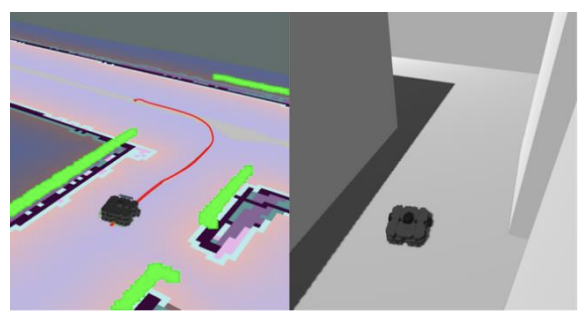
\includegraphics[height=40mm,width=80mm]{./figs/map_base.png}
%      \caption{Imitation learning of path-tracking}\label{fig:mapbase}
% \end{figure}
\begin{figure}[h!]
    \centering
    %  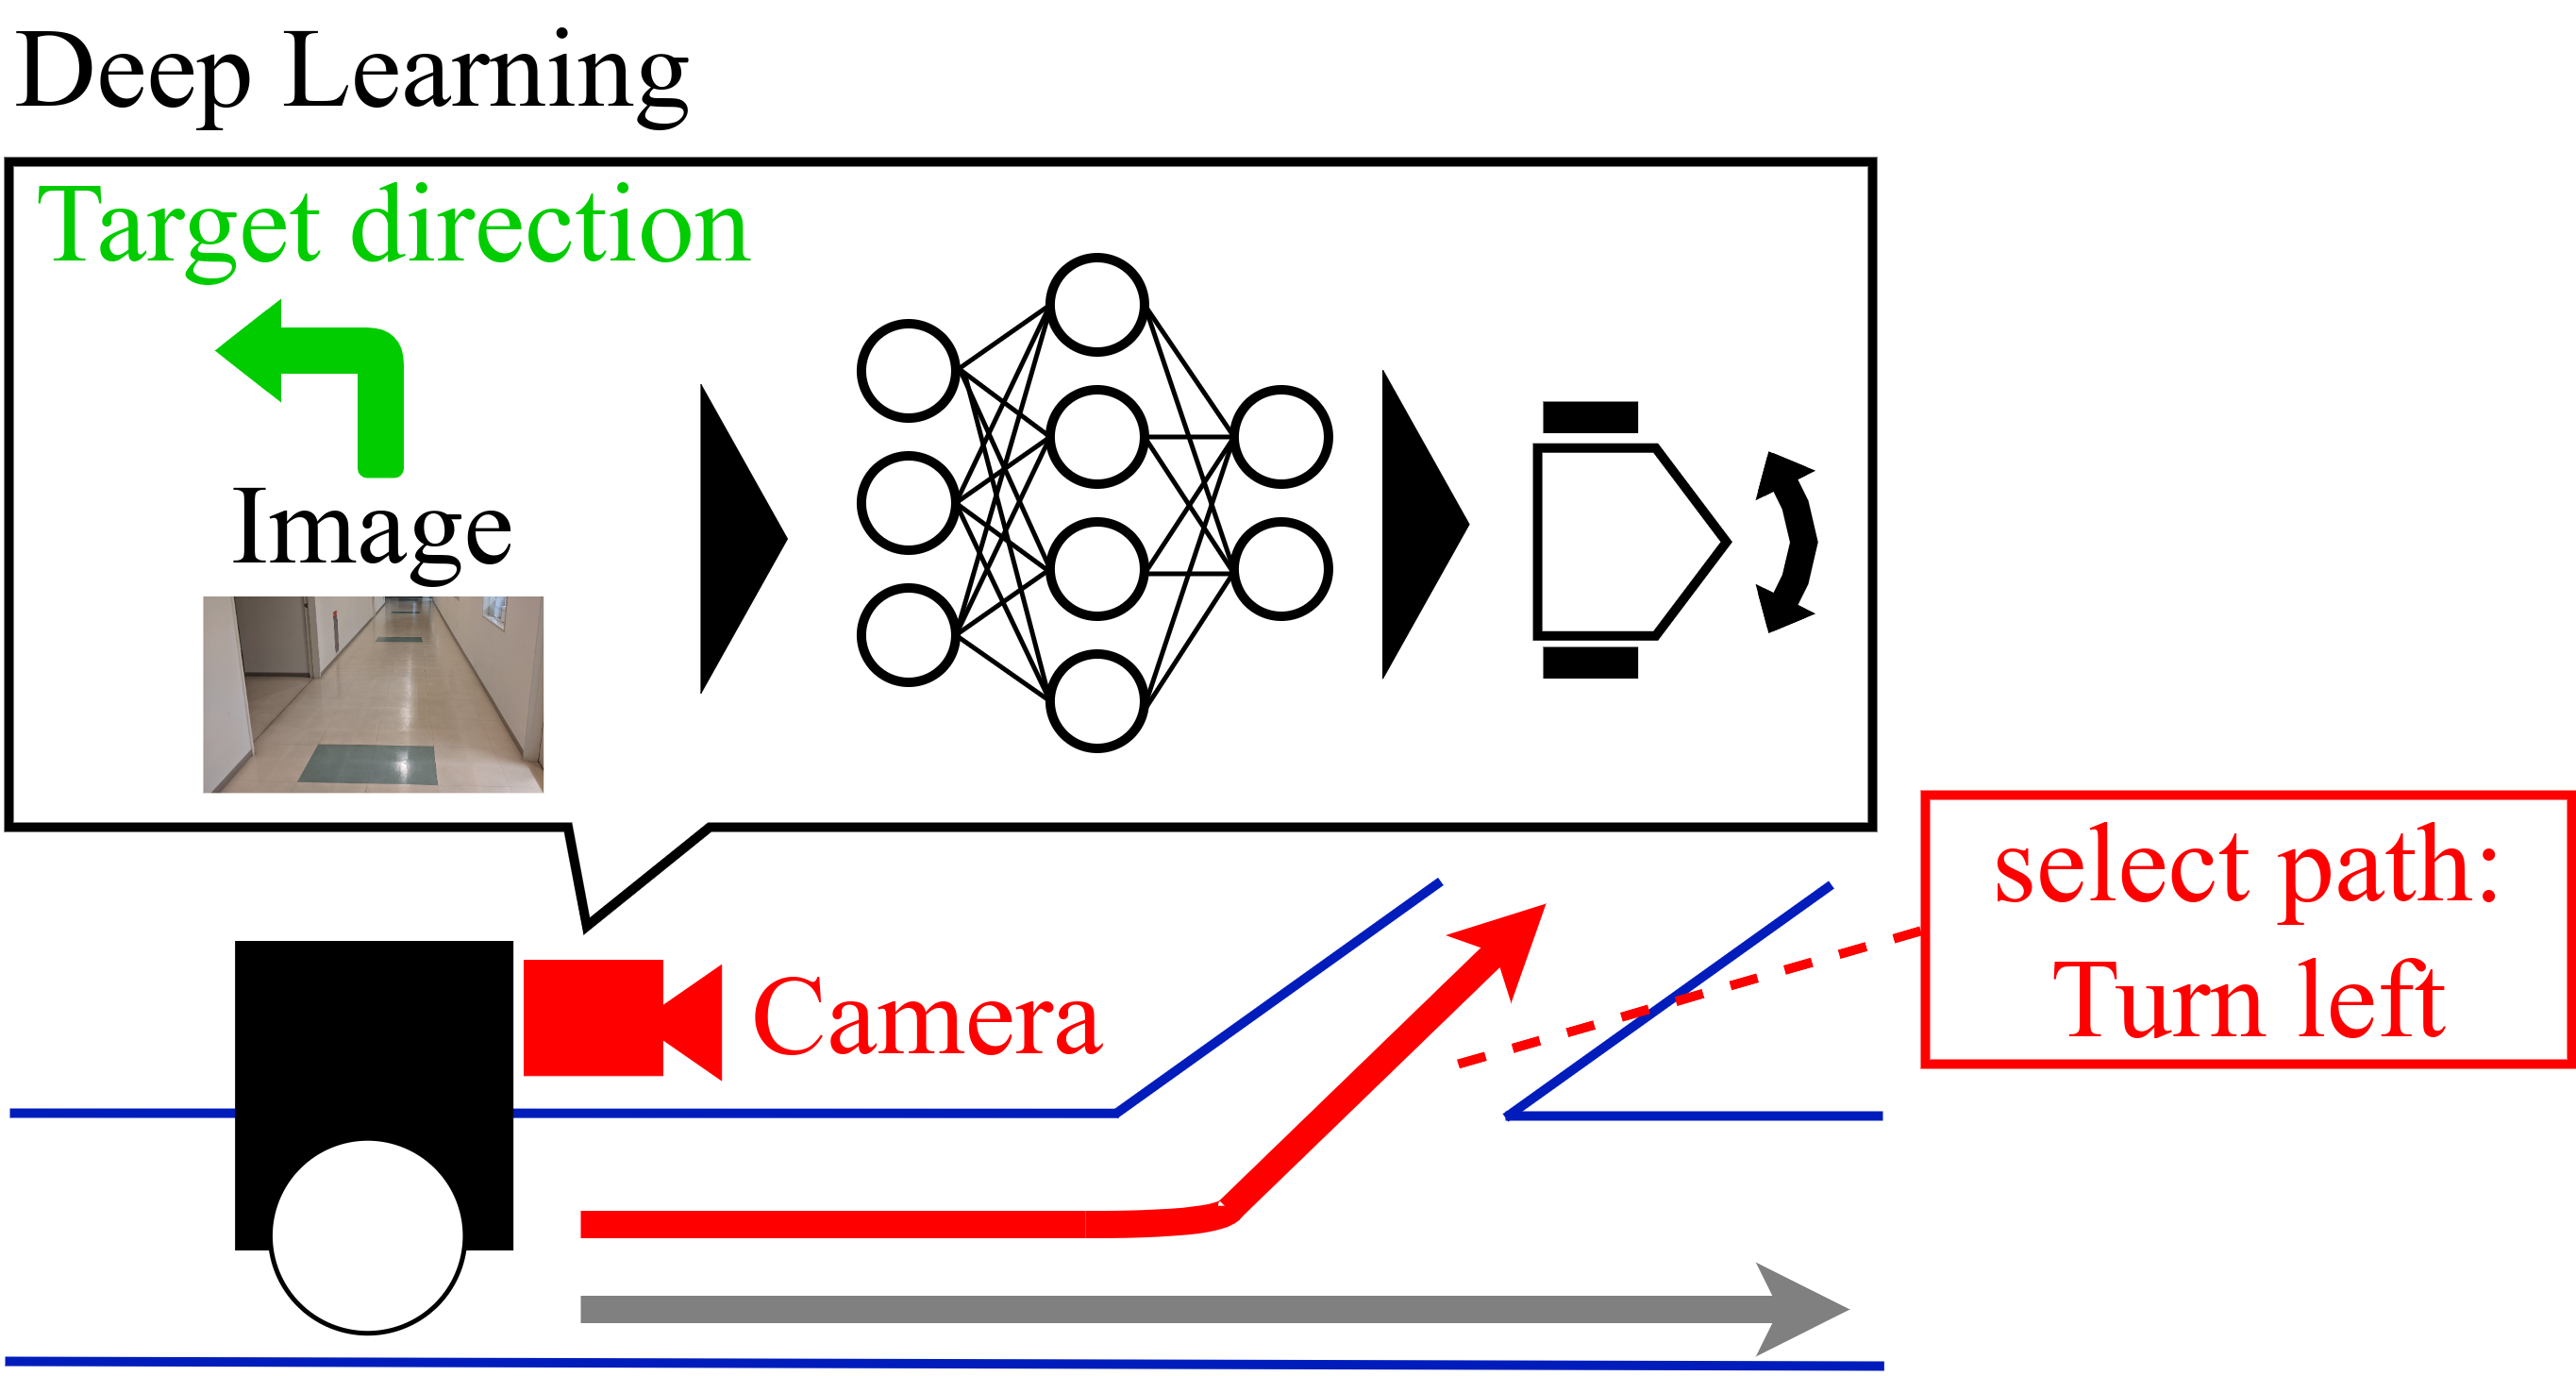
\includegraphics[height=33mm,width=78mm]{./figs/camera_base.png}
     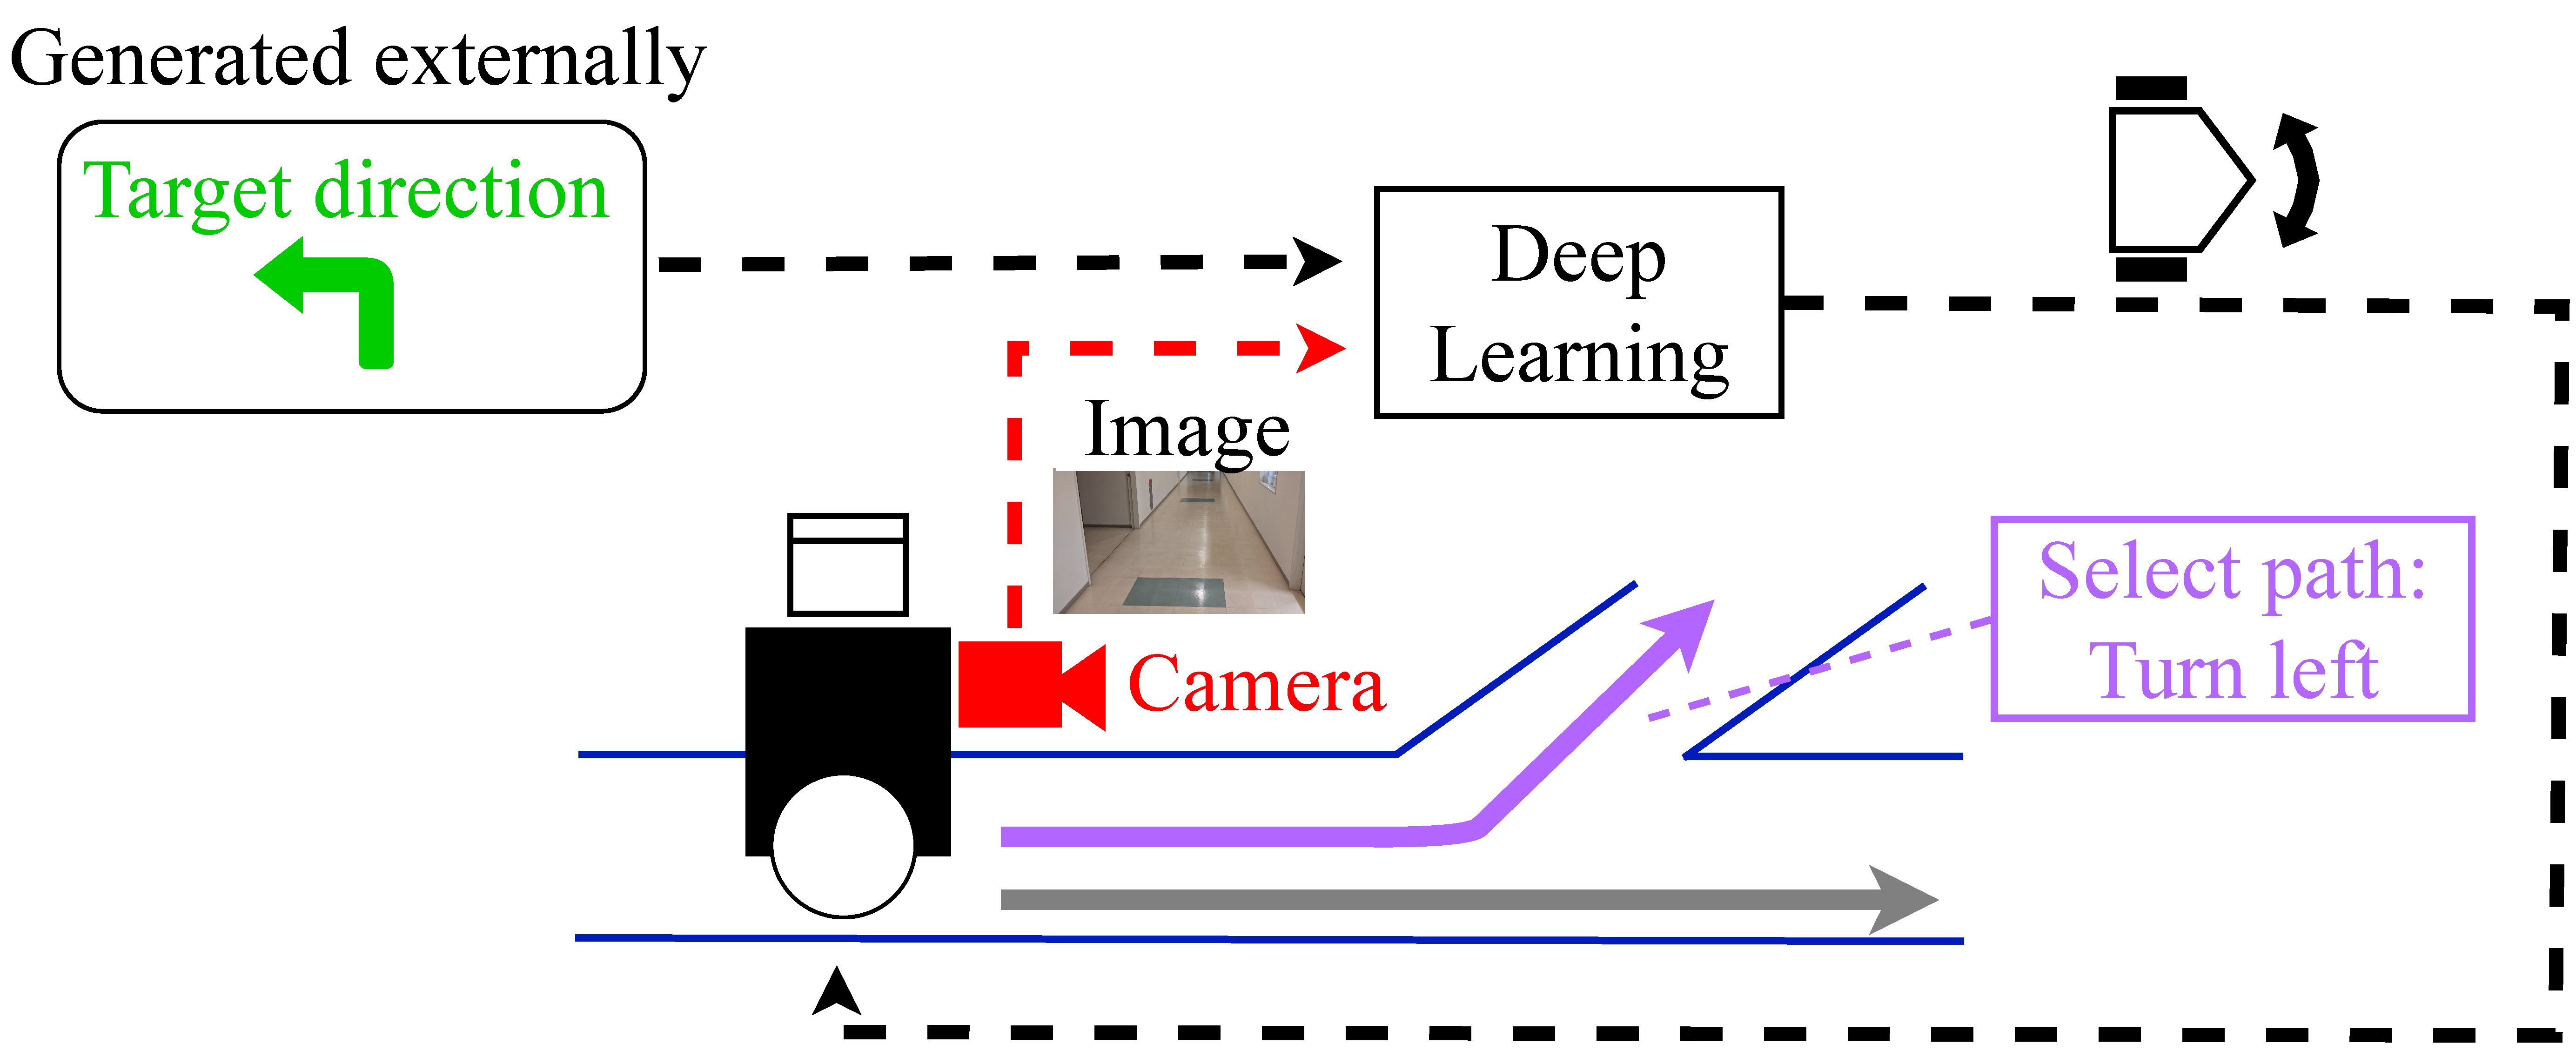
\includegraphics[height=35mm,width=78mm]{./figs/lergan.pdf}
     \caption{Path selection and following behavior based on camera images and
     target direction by imitation learning.}\label{fig:camera_base}
\end{figure}
\begin{figure*}[t]
    \centering
     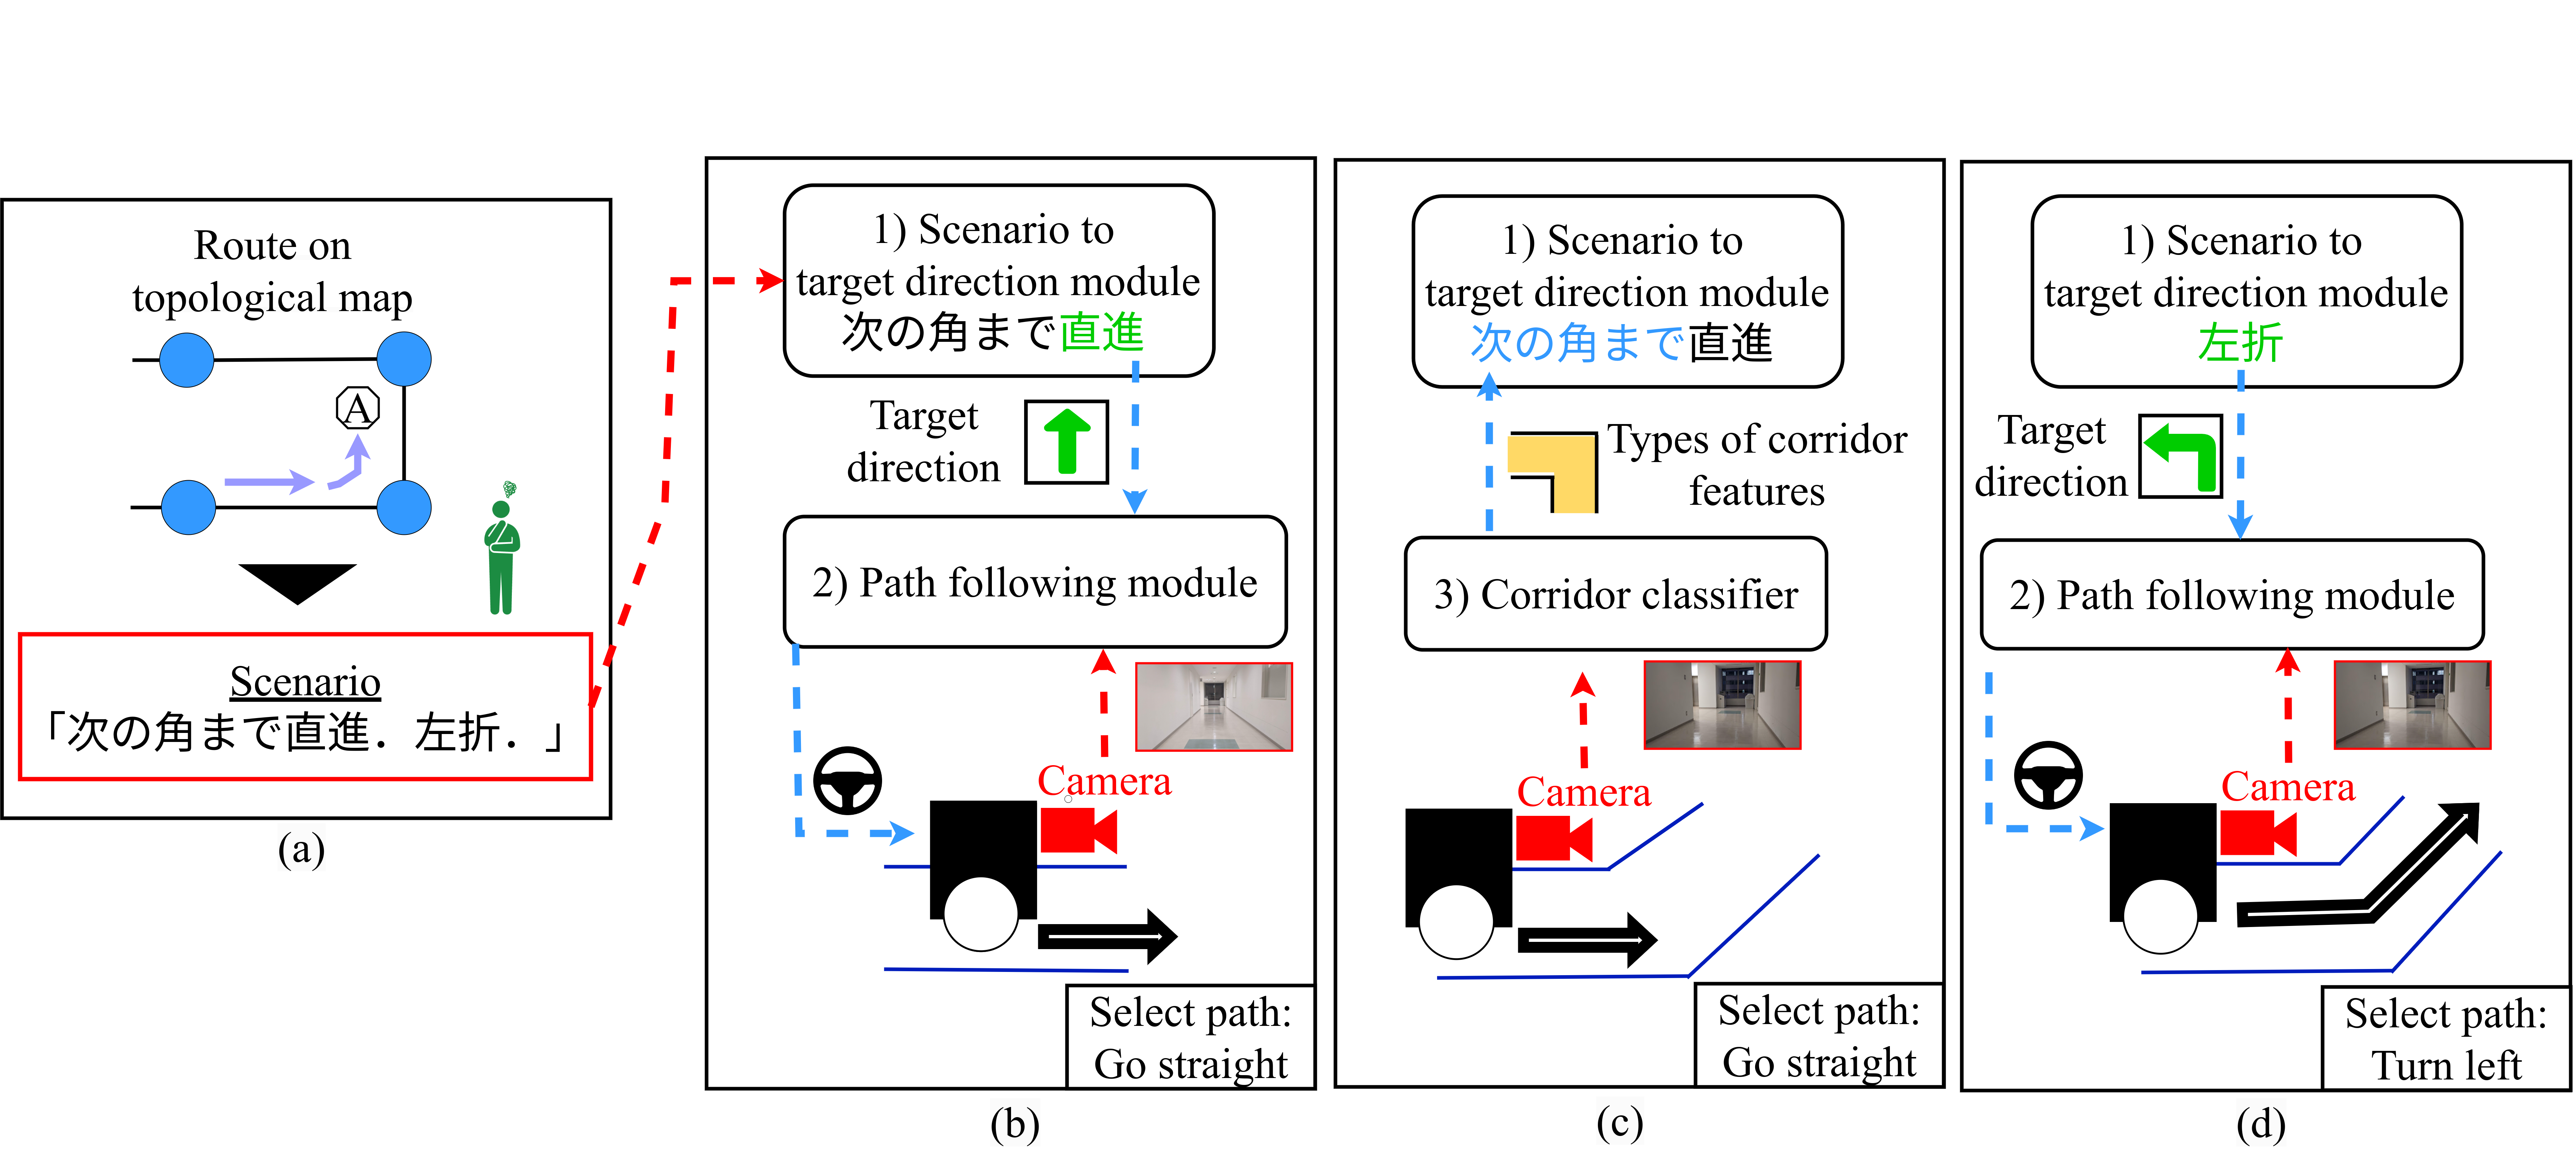
\includegraphics[height=60mm,width=160mm]{./figs/absv3.png}
    %  
\includegraphics[height=50mm,width=160mm]{./figs/absv3_5.pdf}
     \caption{Overview of proposed method}\label{fig:system}
\end{figure*}
\section{提案手法}
提案する手法では,人間が作成した「次の角まで直進.左折」などのシナリオから
指示される道順に従い,カメラ画像に基づいて目的地まで自律移動する.
% この手法の特徴として,目的地までの自律移動に,LiDARなどを用いて事前に
% 作成したメトリックマップを必要としないことが挙げられる.
本章では手法の流れについて述べた後,それぞれのモジュールの詳細を述べる.
\par
Fig.\ref{fig:system}に提案手法の概要と一連の流れを示す.
提案手法は,1)シナリオを分解し,「条件」と「行動」を抽出するモジュール
2)カメラ画像と目標方向に基づく経路追従モジュール
3)シナリオの「条件」の判定に用いる,通路の特徴を分類する通路分類器
の3つのモジュールで構成される.
はじめに,人間が作成したシナリオがモジュールへ入力される.
自律移動時はロボットに取り付けたカメラから得た画像データを入力とする

% システムは,ロボットに取り付けたカメラから得た画像データと,
% トポロジカルマップを基に人間が作成したシナリオを入力とし,
% \begin{enumerate}
%     \item [1)] シナリオの条件を満たしたかの判定に用いる,通路の特徴を分類する通路分類器
%     \item [2)] シナリオを解釈し,目標方向へ変換して出力するモジュール
%     \item [3)] カメラ画像と目標方向に基づく経路追従モジュール\
% \end{enumerate}

一連の流れを下記に示す
\begin{enumerate}
    \item [(a)] トポロジカルマップ上の経路から
    人間が「条件」と「行動」で構成される経路の表現(シナリオ)を生成する.
    生成されるシナリオ:「次の角まで直進.左折.」
    \item [(b)] 生成されたシナリオを句点ごとに区切り,
    次に「条件」と「行動」を抽出する.
    1つ目の区切りでは条件:次の角まで,行動:直進が登録される
    経路追従モジュールは,カメラ画像に基づいて,経路に沿って直進する.
    \item [(c)] 角の部分に到達し,カメラ画像に基づく通路分類の結果が角となり,
    「次の角まで」というシナリオの条件が満たされた場合,2つ目の区切りへ遷移する.
    \item [(d)]2つ目の区切りでは行動:左折が登録され,
    経路追従モジュールは経路に沿って左折する.
\end{enumerate}
% Fig.\ref{fig:system}(a)でトポロジカルマップとこのマップ上の経路から
% 人間が「条件」と「行動」で構成したシナリオを生成する.
% ここで生成されるシナリオは「次の角まで直進.右折.」となる.
% Fig.\ref{fig:system}(b)では,生成されたシナリオを1)の
% シナリオを解釈するモジュールが分解し,「次の角まで直進」が抽出される.

% この入力されたシナリオを2)のモジュールが「条件」と「行動」に分解し,
% この行動を目標方向へ変換して出力する.
% 具体的には,1)の通路分類器から「三叉路」という分類結果が得られるまで,
% 「直進」の目標方向を出力し,3)の経路追従モジュールへ与える.
% 3)の経路追従モジュールはカメラ画像と与えられた目標方向をもとに,
% 「直進」の経路を追従する.
% 1)の通路分類器から「三叉路」の分類結果が得られた場合,
% 2)のモジュールは次に「右折」の目標方向を出力し,
% 3)のモジュールは経路に沿って右折する.



\subsection{カメラ画像と目標方向に基づく経路追従}
カメラ画像と目標方向に基づいて,
経路を追従するモジュールについて述べる.
このモジュールは,地図を用いたルールベース制御器の出力を模倣するように学習して,
カメラ画像に基づいた経路追従行動を獲得する\cite{haruyama2022}\cite{fujiwara2023}.
これにより,学習後はRGBカメラのみのセンサ入力で経路追従が可能である.
\par
Fig.\ref{fig:learning}に経路追従モジュールのシステムを示す.
学習時は,2D-LiDARやオドメトリ,事前に作成したメトリックマップに
基づいたルールベース制御器(ROS Navigation Stack\cite{ros-navigation})によって,
設定した経路を走行する.
その際,入力をカメラ画像,目標方向,
出力をヨー方向の角速度(地図を用いたルールベース制御器が出力)として,0.2秒周期でデータセットに加える.
さらに,バッチサイズを8として教師データをデータセットから抽出し,
0.2秒の周期でオンラインで学習する.
このデータセットにデータを追加,データの抽出,学習の1連の流れを1ステップとする.
ここでの目標方向は,地図に基づいたルールベースの制御器から出力される信号を用いる.
データセットの収集には,藤原ら\cite{fujiwara2023}が提案した
% \cite{fujiwara2023}
% [藤原]
データセットの不均衡の改善,
学習時における積極的な蛇行といった最も経路追従の成功率の高い手法を採用する.
\par
学習後,カメラ画像と
後述するシナリオを解釈し,変換するモジュールから目標方向を与え,
出力されるヨー方向の角速度によりロボットを制御する.
このとき,並進速度には0.2m/sの一定の値を与える.
% \cite{haruyama2022}\cite{fujiwara2023}では
% [春山][藤原]
% 前報では
% 学習後も,
% 地図に基づいたルールベース制御器から生成される目標方向を用いていた.
% 本稿では,学習後で用いる目標方向を,
% 次の節で述べるシナリオに基づくナビゲーションから生成する.
% なお学習器のネットワークは
% \cite{haruyama2022}\cite{fujiwara2023}
% % [春山][藤原]
% と同様の構成を用いる.
\begin{figure}[htbp]
    \centering
     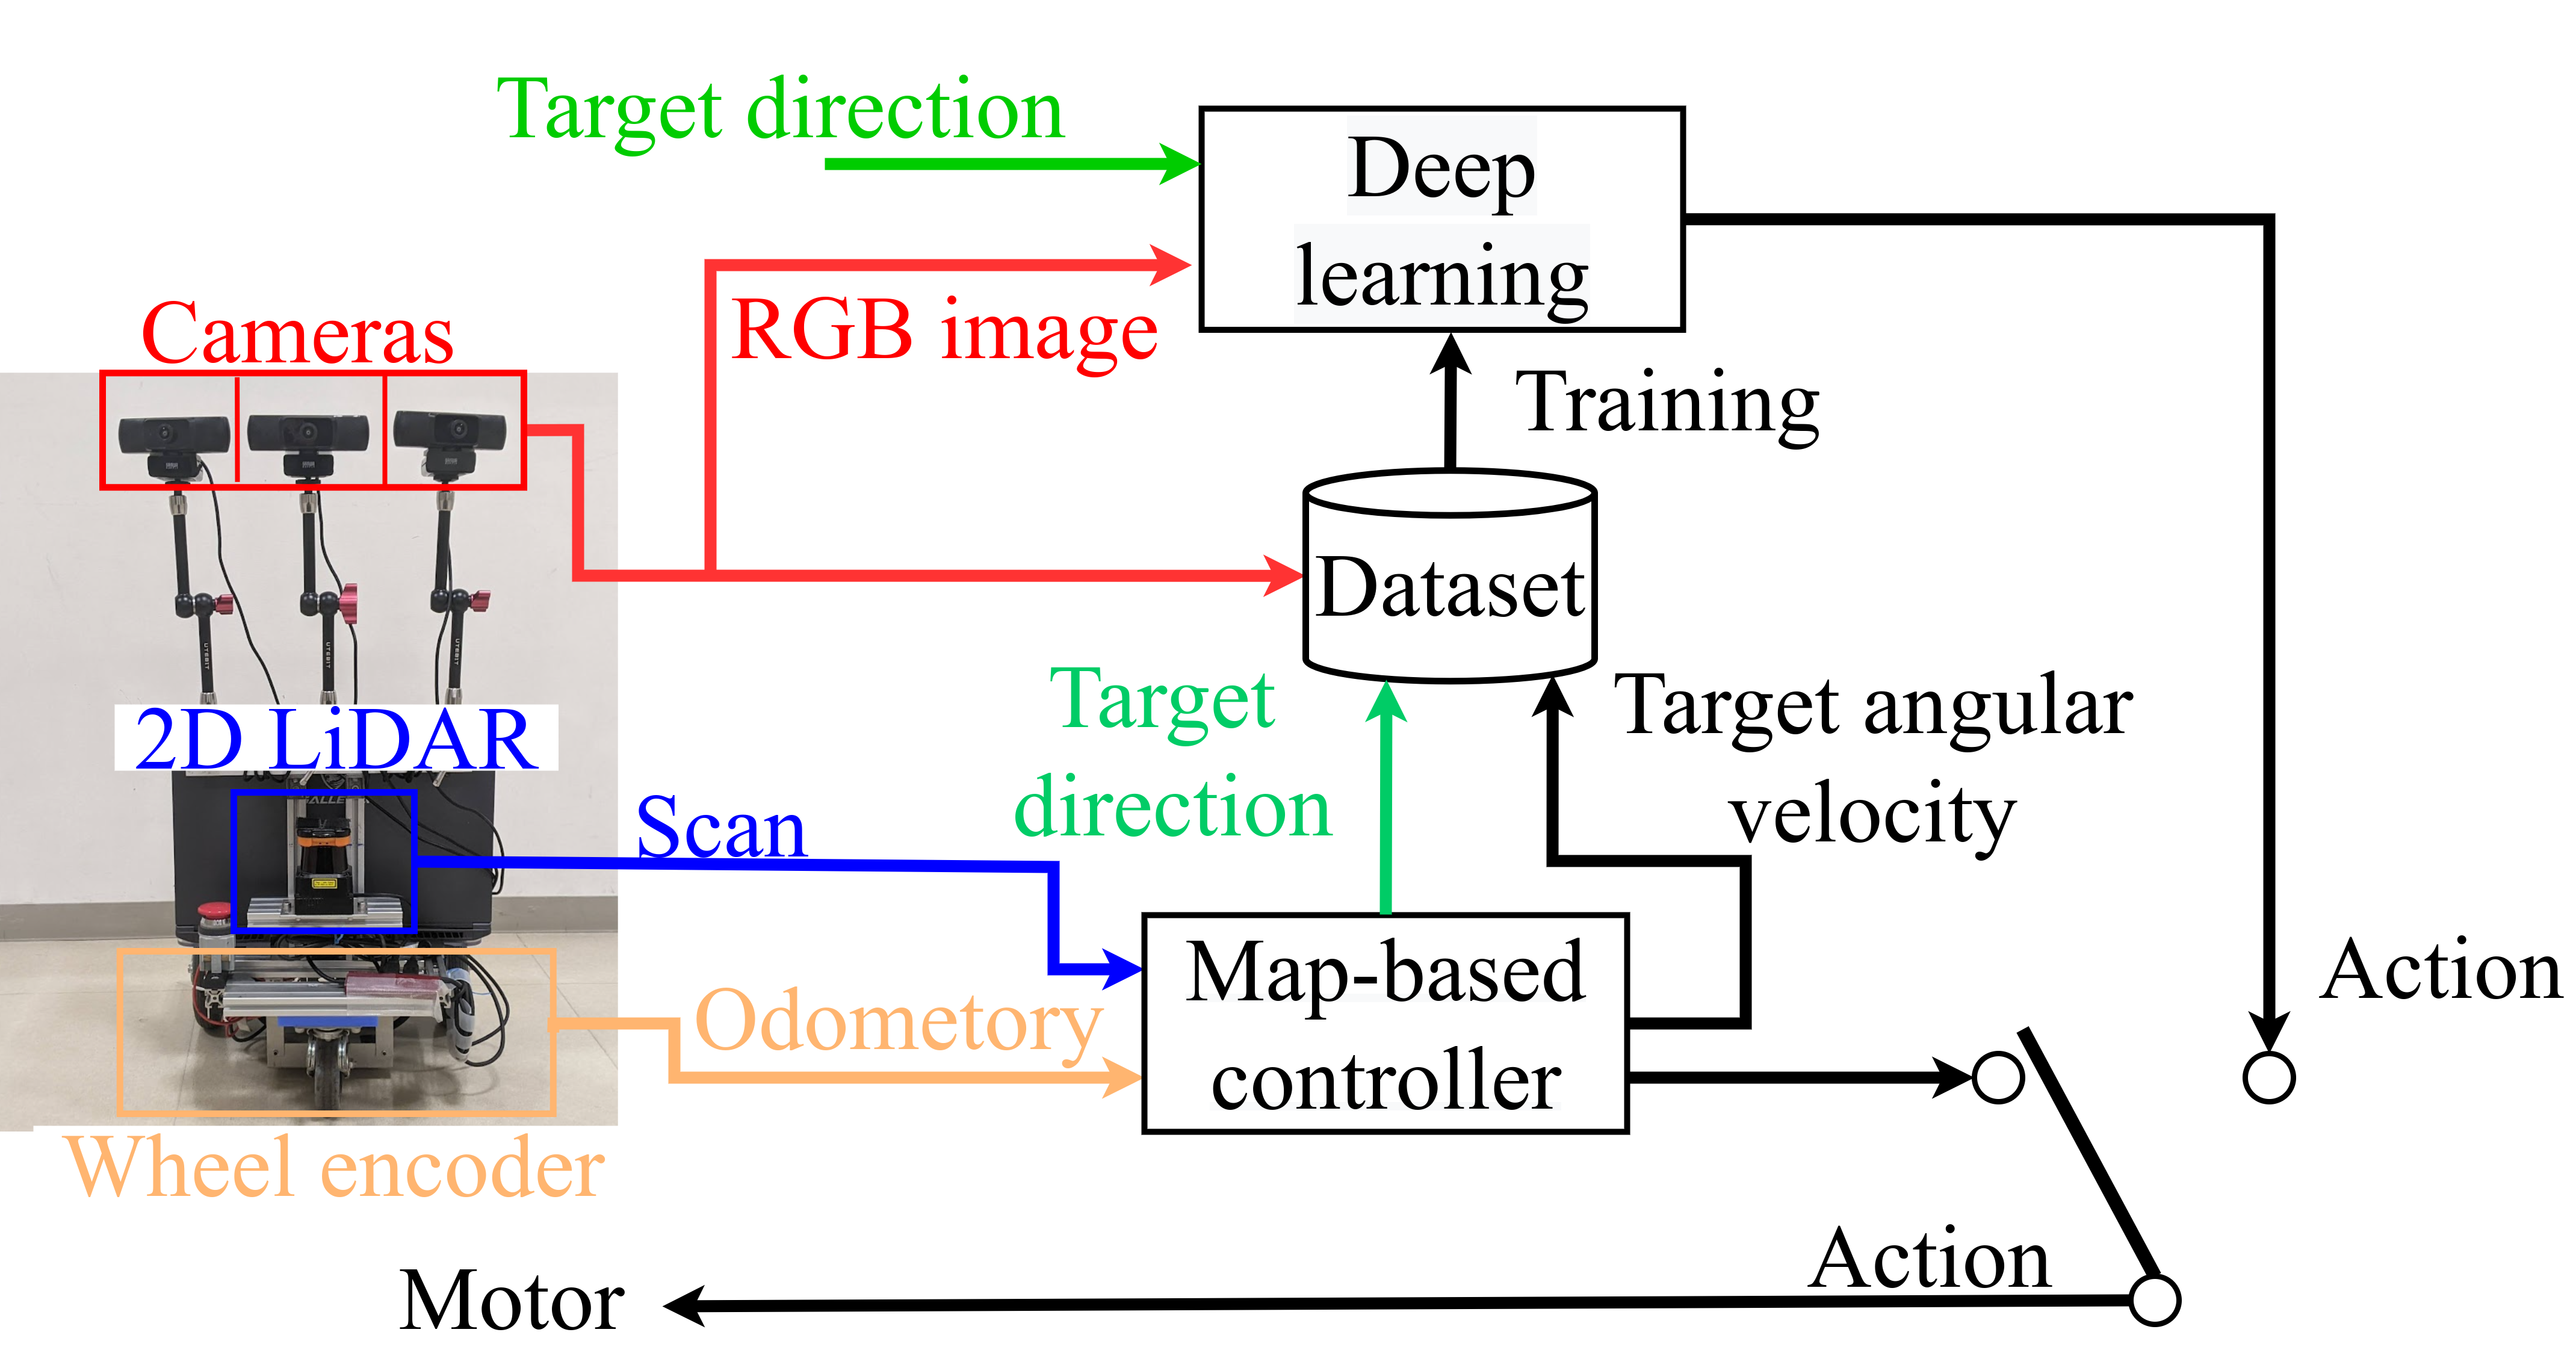
\includegraphics[height=45mm,width=80mm]{./figs/learning_gamma.png}
     \caption{Imitation learning system with target direction}\label{fig:learning}
\end{figure}
\subsection{シナリオから目標方向への変換}
シナリオから経路追従モジュールが必要とする目標方向を出力するモジュールについて述べる.
このモジュールはトポロジカルマップから作成された
シナリオから「突き当りまで」という「条件」や
「直進」などの「行動」を解釈し,単語で構成された経路を目標方向へ変換して出力する.
後述する分類器と組み合わせることで,目的地までの自律移動に必要な目標方向を,メトリックマップを用いずに,
経路追従モジュールへ与えることを可能とする.
% このナビゲーションは\cite{shimada2020}
% [島田ら]
% で提案された人の道案内情報を収集・分析し,
% そのデータを基にトポロジカルマップの形式とシナリオ(経路の表現)を用いて
% ロボットをナビゲーションする手法をベースに構成する.
% ~にトポロジカルマップとシナリオの例を示す.
\par
\begin{figure}[htbp]
    \centering
     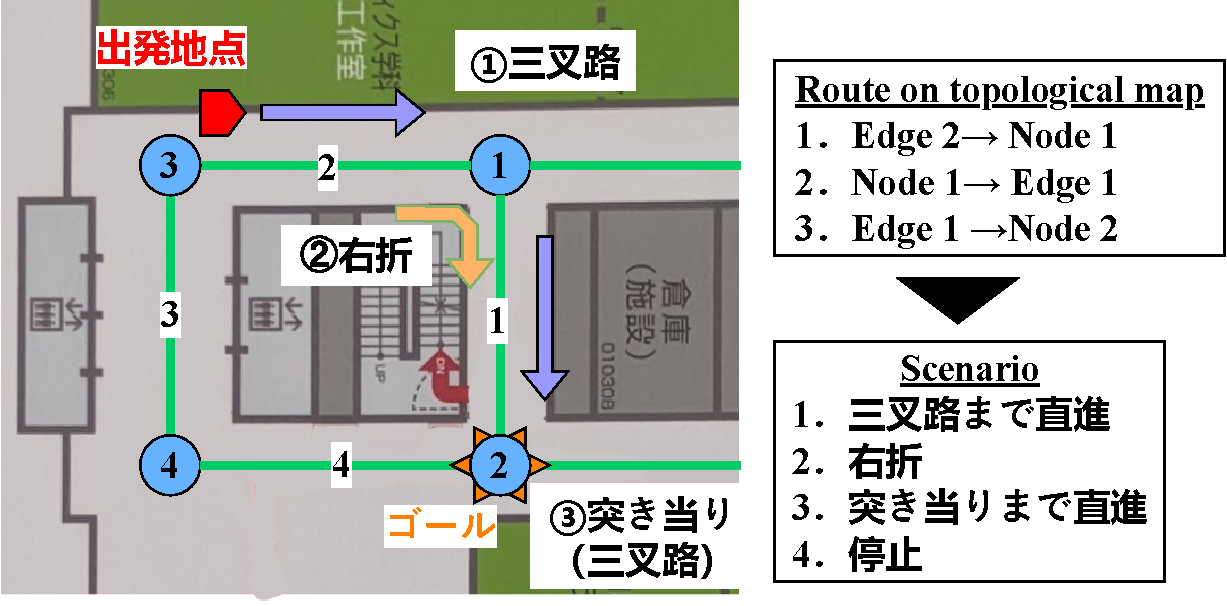
\includegraphics[height=40mm,width=80mm]{./figs/topo2sce.pdf}
     \caption{Example of topological map and generated scenario}\label{fig:topo2sce}
\end{figure}
\par
Fig.\ref{fig:topo2sce}にトポロジカルマップの例とそれを基に生成されるシナリオを示す.
トポロジカルマップは通路の特徴的な箇所に配置されたノード(Fig.\ref{fig:topo2sce}青),
これらをつなぐエッジ(Fig.\ref{fig:topo2sce}緑)で構成される.
ノードはID,通路の特徴,接続されるエッジとその方向のデータが含まれ,
エッジにはIDのデータのみが含まれている.
シナリオはトポロジカルマップ上での目的地までの経路を「条件」と「行動」に関する単語を組み
合わせによって表現したものである.
Fig.\ref{fig:topo2sce}のトポロジカルマップとシナリオを生成する例を示す.
この例では出発地点をエッジ2,目的地をノード2として,エッジとノードを経由していく.
エッジ2からノード2までの経路は
エッジ2からノード1は「三叉路まで」という条件と「直進」という行動,
ノード1からエッジ1は「右折」という行動,
エッジ1からノード1は「突き当り(三叉路)まで」という条件と「直進」の行動で表現される.
これらを統合すると,
最終的に「三叉路まで直進.右折.突き当たりまで直進.停止」
が生成される.\par
次に生成されたシナリオを目標方向として変換する方法を述べる.
目標方向への変換では
シナリオを句点ごとに分解後,「条件」と「行動」を示す言葉を抽出し,
以下の項目に分けて登録する.\\
% \begin{enumerate}
%     \item [1)] 通路の特徴
%     \item [2)] 順番
%     \item [3)] 方向
%     \item [3)] 方向
% \end{enumerate}
1)通路の特徴\\
2)順番\\
3)方向\\
4)行動\\
シナリオの例は句点ごとに
三叉路まで直進/ 
右折/ 
突き当たりまで直進/ 
停止/ 
と区切られる.
1つ目の区切りでは\\
1)通路の特徴:三叉路\\
4)行動:直進\\
2つ目の区切りでは\\
4)行動:右折\\
が登録される.
この一連の作業を末尾の区切りである「停止」が登録されるまで行う.
ここで登録される「行動」を目標方向として,前述の経路追従モジュールへ与える.
目標方向のデータ形式をTable \ref{tab:target}に示す.
ここで,「三叉路まで」といった条件を満たしたかの判定は後述する通路分類器を用いて行う.
\begin{table}[]
    \centering
    \caption{Target direction and data for imitation learning}\label{tab:target}
    \begin{tabular}{|c|c|}
    \hline
    Target direction & Data        \\
    \hline
    Go straight   & {[}1,0,0{]} \\
    Turn left   & {[}0,1,0{]} \\
    Turn right   & {[}0,0,1{]} \\
    Stop   & {[}0,0,0{]}\\
    \hline
    \end{tabular}
    \end{table}

% \par
% 島田らは1)の機能の他に2)通路の特徴を検出する機能
% 3)経路に沿って通路を走行する2つの機能を開発している.
% しかし,\cite{shimada2020}\cite{hara2022}
% % [島田][原]
% の手法では2)と3)にLiDARや全天球カメラのセンサ入力を
% 必要としている.
% そのため,本稿では.
% 2)の通路の特徴検出を,次の小節で述べるカメラ画像による手法,
% 3)に関しては前述した経路選択機能をもつ学習器へ変更している.

\subsection{通路の特徴を分類する通路分類器}
シナリオで用いる「条件」を満たしたかの判定に必要な通路の特徴を,
カメラ画像と深層学習によって分類する通路分類器について述べる.
このモジュールは
RGBカメラのみのセンサ入力で通路の特徴を分類することが可能である.
通路分類器の概要をFig.\ref{fig:lrcn}に示す.通路分類器は
フレーム数16の連続した画像データ(画像サイズは64×48)
を入力とし,通路の特徴の分類を出力する.
通路の特徴の分類は島田らの手法\cite{shimada2020}に倣い,
Fig.\ref{fig:intersection}に示した8つとする.
この通路分類器のネットワークアーキテクチャは
Dhaivatらが提案するCNNとLSTMを組み合わせたLRCN\cite{lrcn}を参考として構築した.
なおシステムでは,CNNアーキテクチャにMobileNetV3-Large\cite{v3}を用いている.
% シーケンスデータのフレーム数は16 

\begin{figure}[h!]
    \centering
     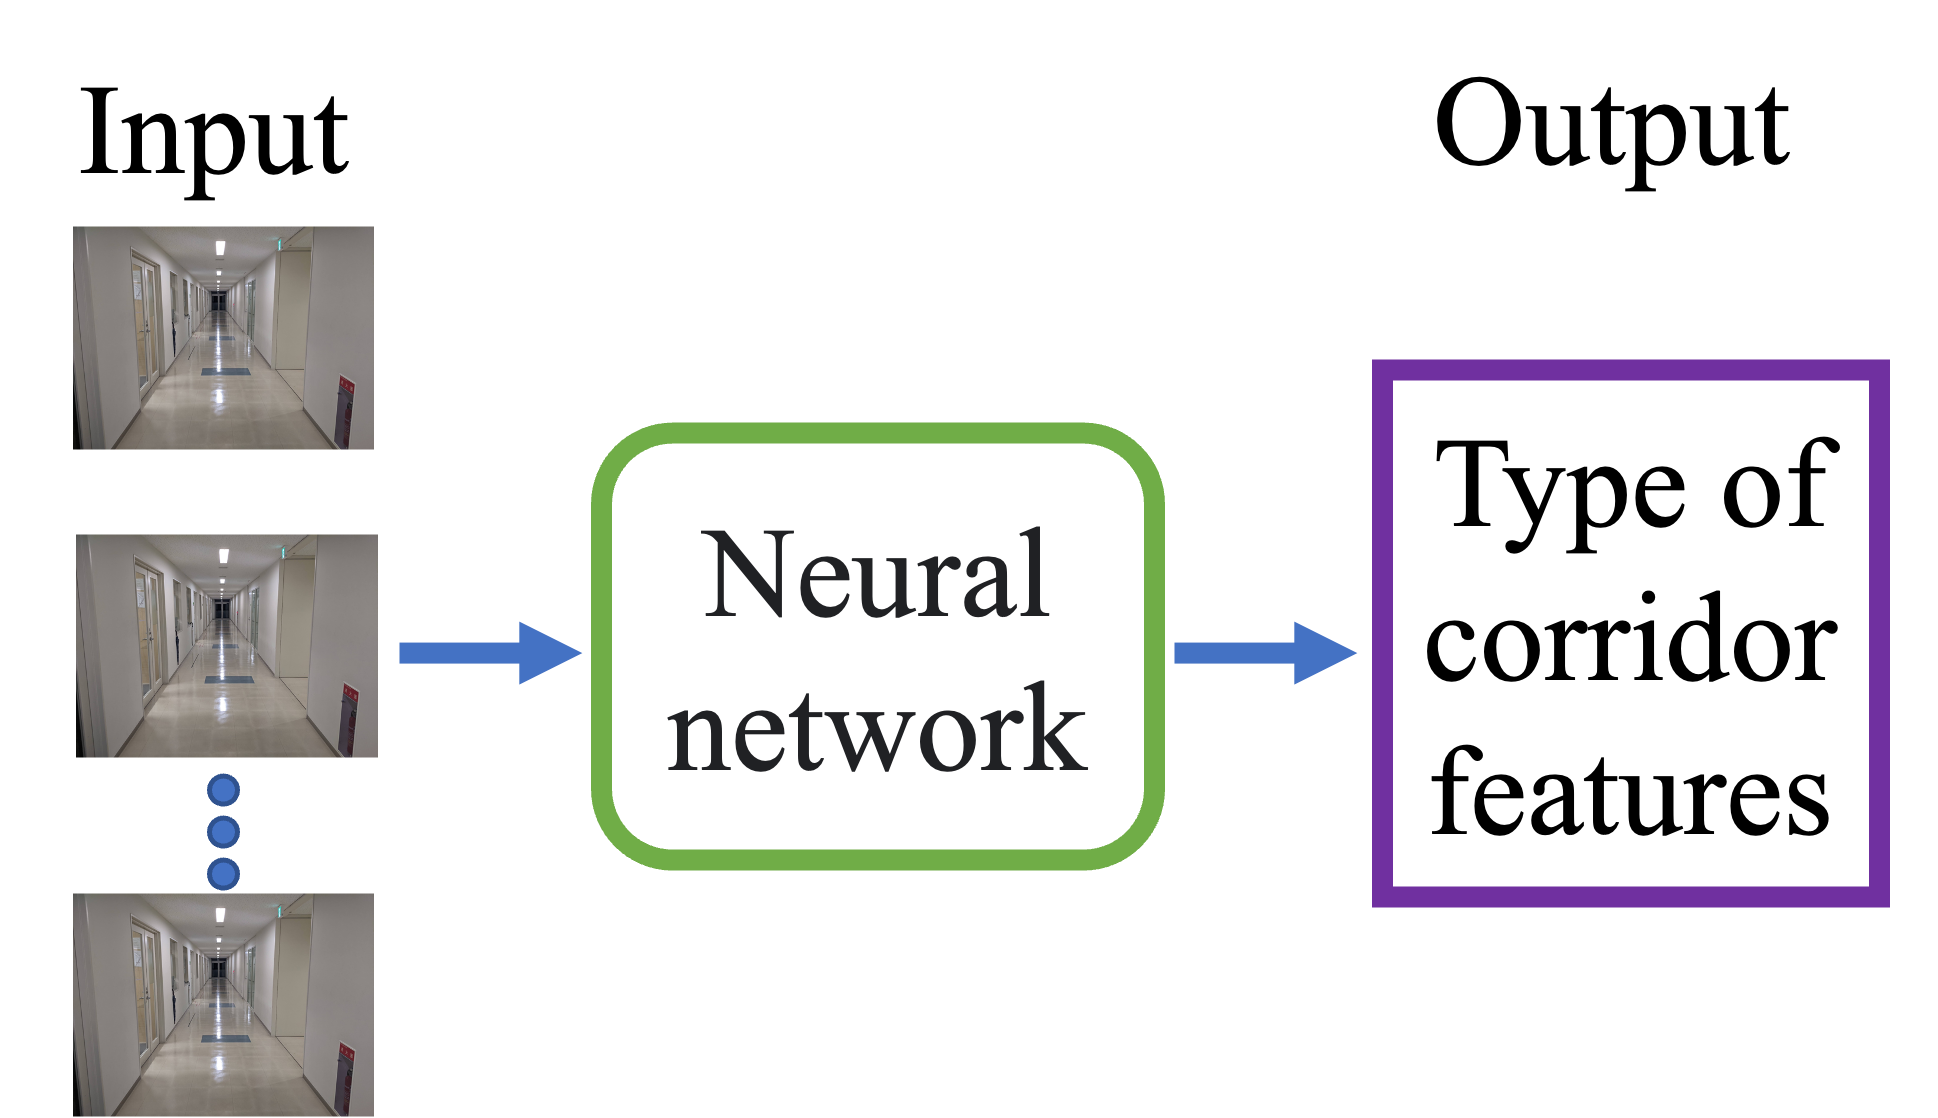
\includegraphics[height=30mm,width=70mm]{./figs/LRCN_gai.png}
     \caption{Types of corridor features classifier overview}\label{fig:lrcn}
\end{figure}
\begin{figure}[h!]
    \centering
     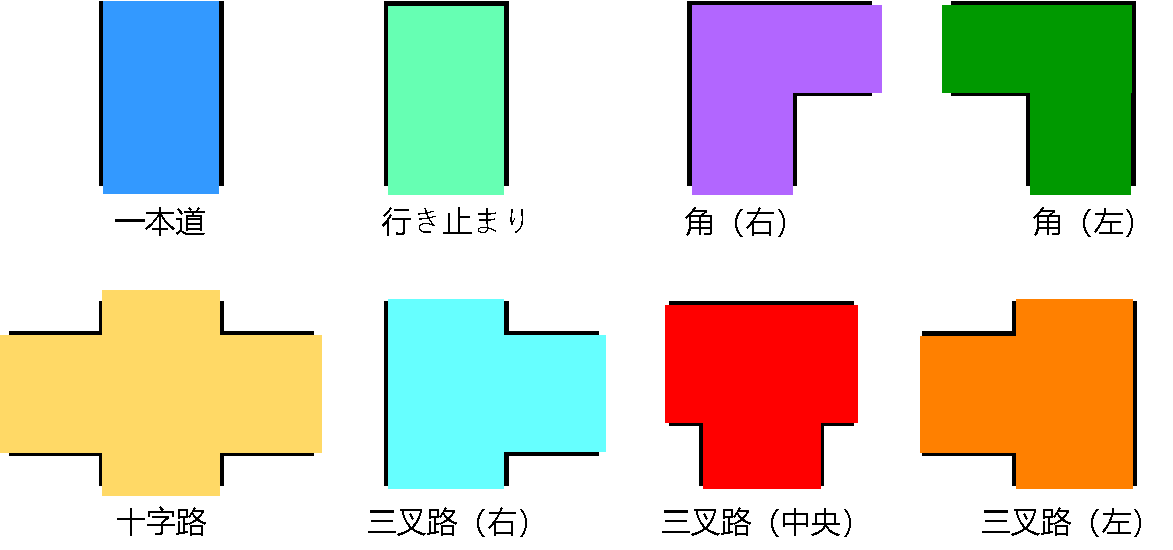
\includegraphics[height=30mm,width=70mm]{./figs/corridor.pdf}
     \caption{Types of corridor features}\label{fig:intersection}
\end{figure}
\par
次に分類器のデータセットの作成について述べる.
データの作成では,地図に基づいたルールベース制御器によって経路を走行し,
その際,フレーム数16の連続したカメラ画像と
通路の分類ラベルを1組とし,0.125秒周期でデータセットへ加える.
その際,分類ラベルのアノテーションは,Fig.\ref{fig:map2label}に示す
地図上で対応した分類ラベルを生成する機能を追加した地図に基づいた
ルールベース制御器の出力を用いて,自動的に行う.
\begin{figure}[h!]
    \centering
     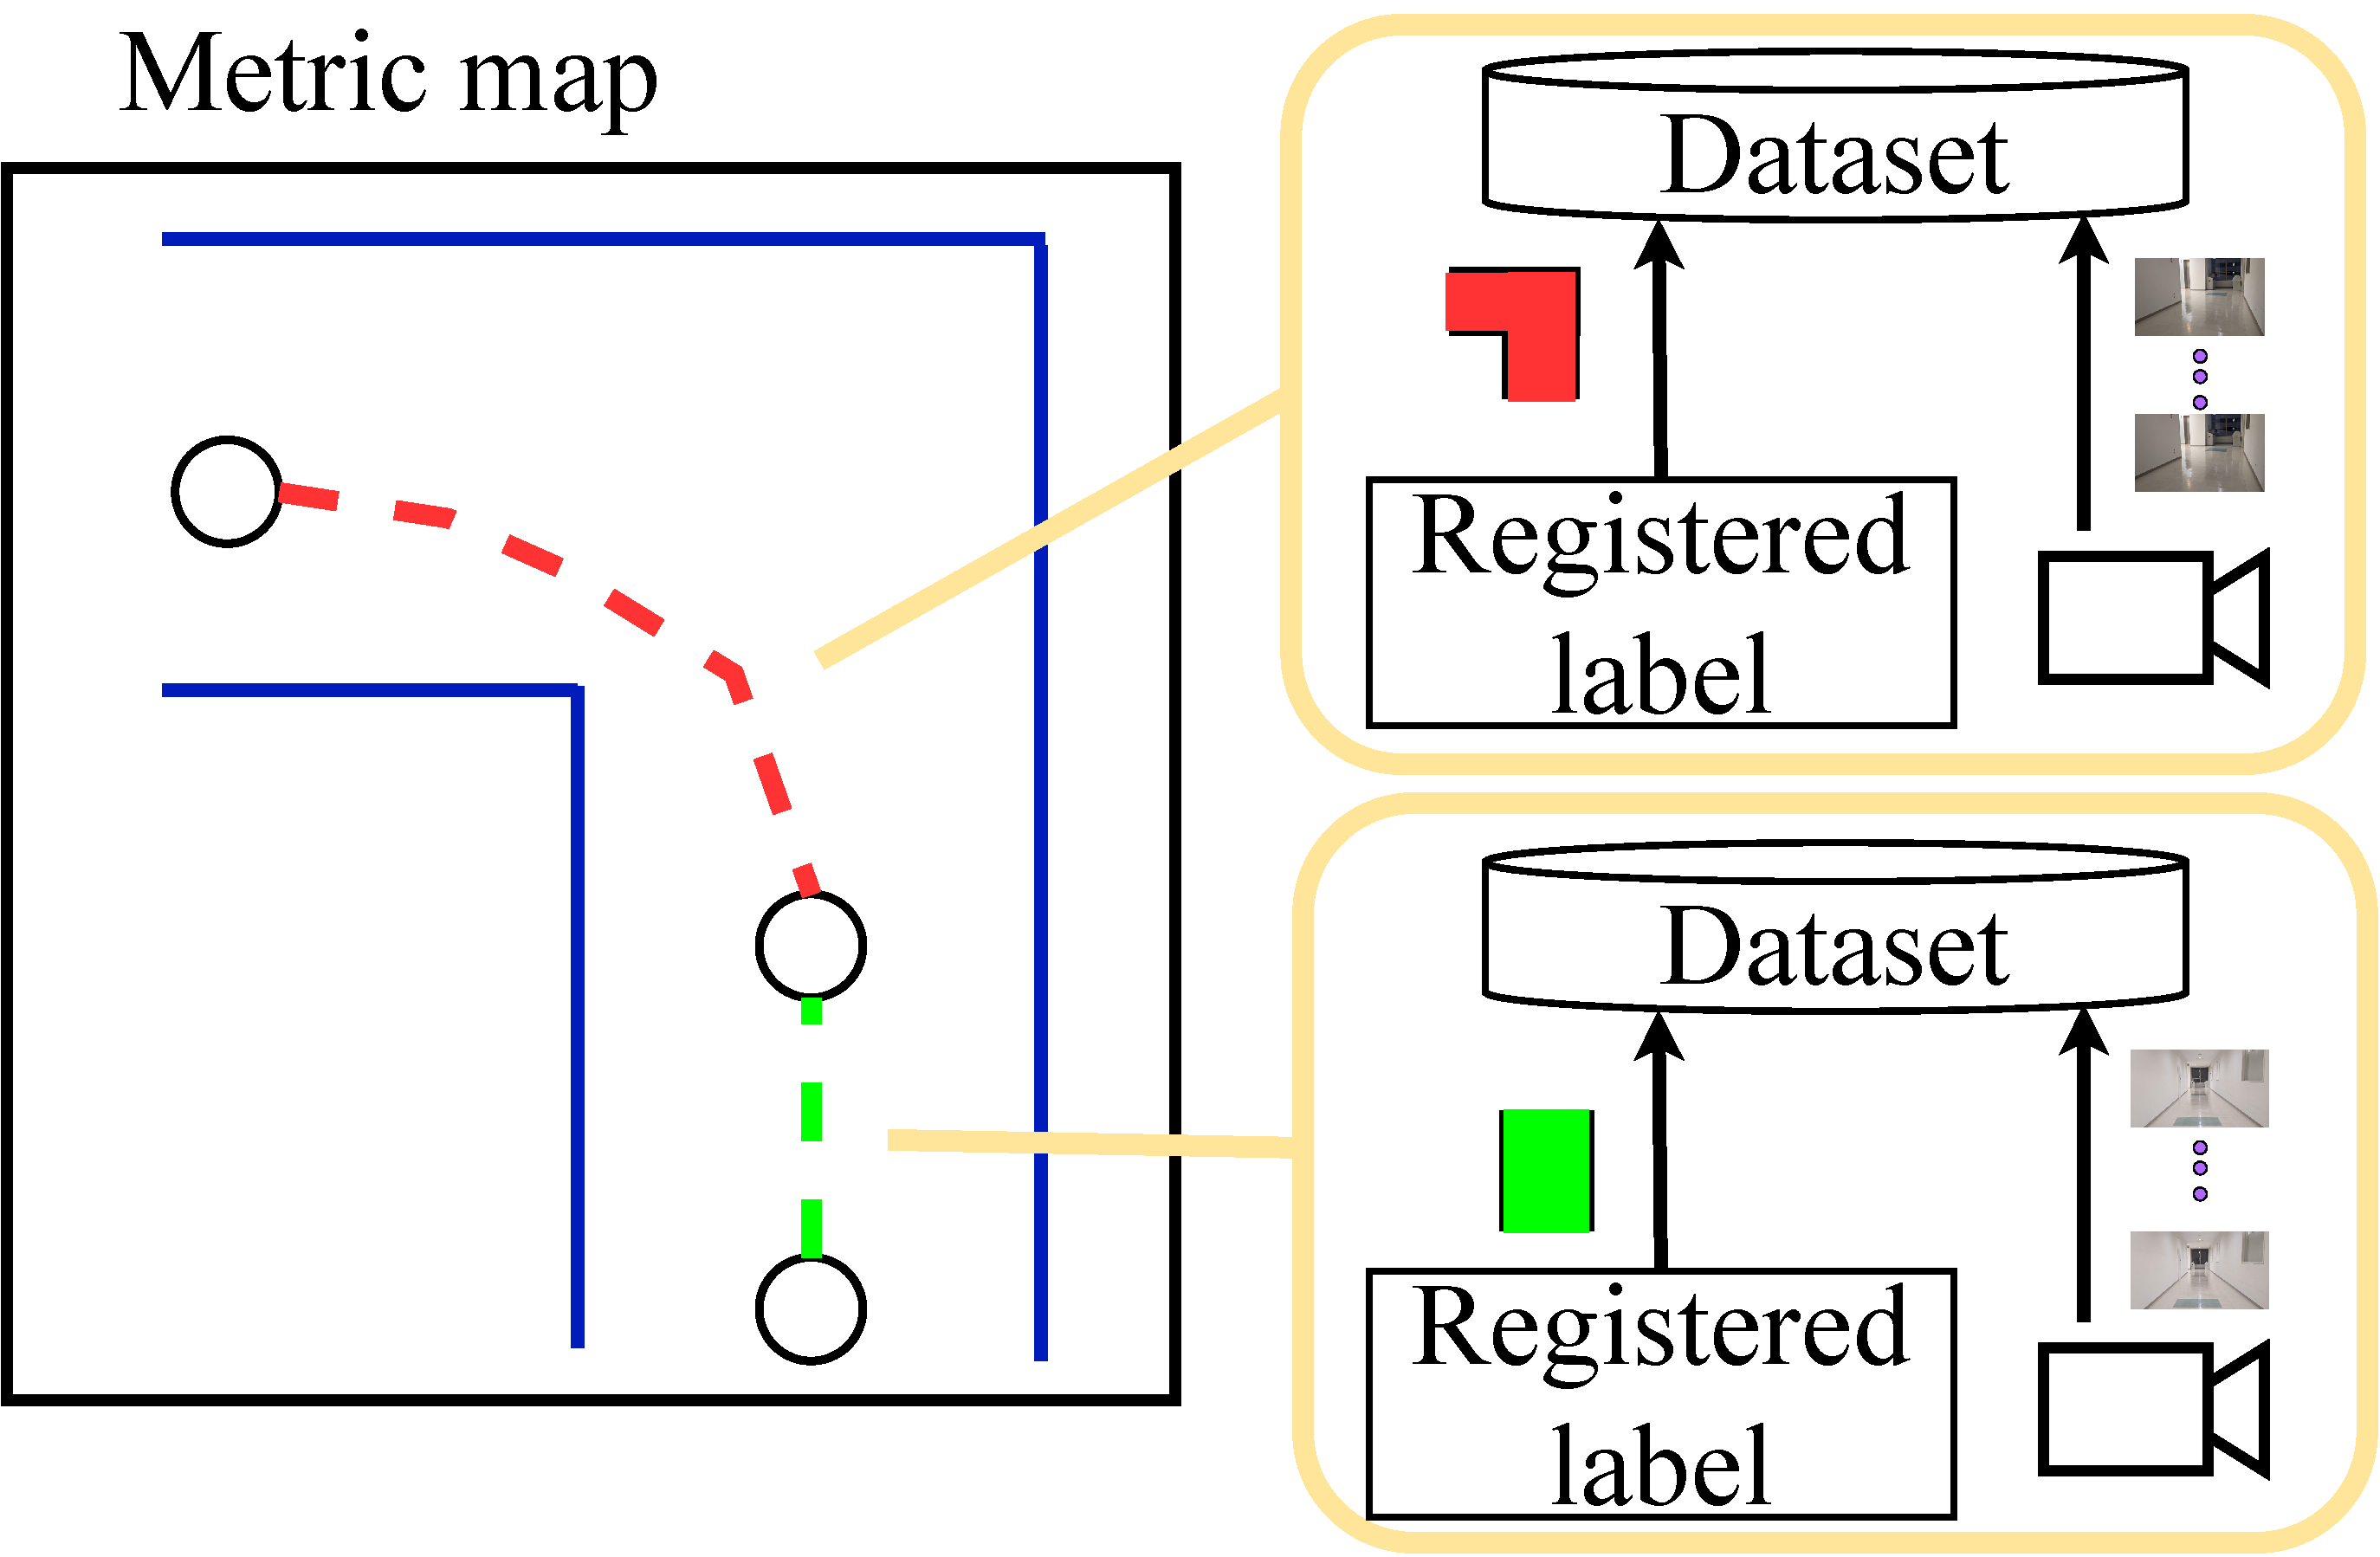
\includegraphics[height=40mm,width=80mm]{./figs/map_label.pdf}
     \caption{Types of corridor features}\label{fig:map2label}
\end{figure}
\par
学習に用いるデータセット内で,各クラスのデータ数が大きく異なる不均衡データは,
分類に大きな影響を与える
\cite{hukin}
とされている.
そのため,本稿では学習する際に,データセット内のクラス間のデータ数によって
重み付けを行うコストアプローチ\cite{cost}を導入している.

\section{実験}
実ロボットを用いて,
提案するカメラ画像とシナリオに基づく経路追従手法により,
ロボットが目的地へ到達可能であるか検証する.

\subsection{実験装置}
実験にはFig.\ref{fig:gamma}で示すカメラを3つ搭載したロボットを使用する.
\begin{figure}[htbp]
    \centering
     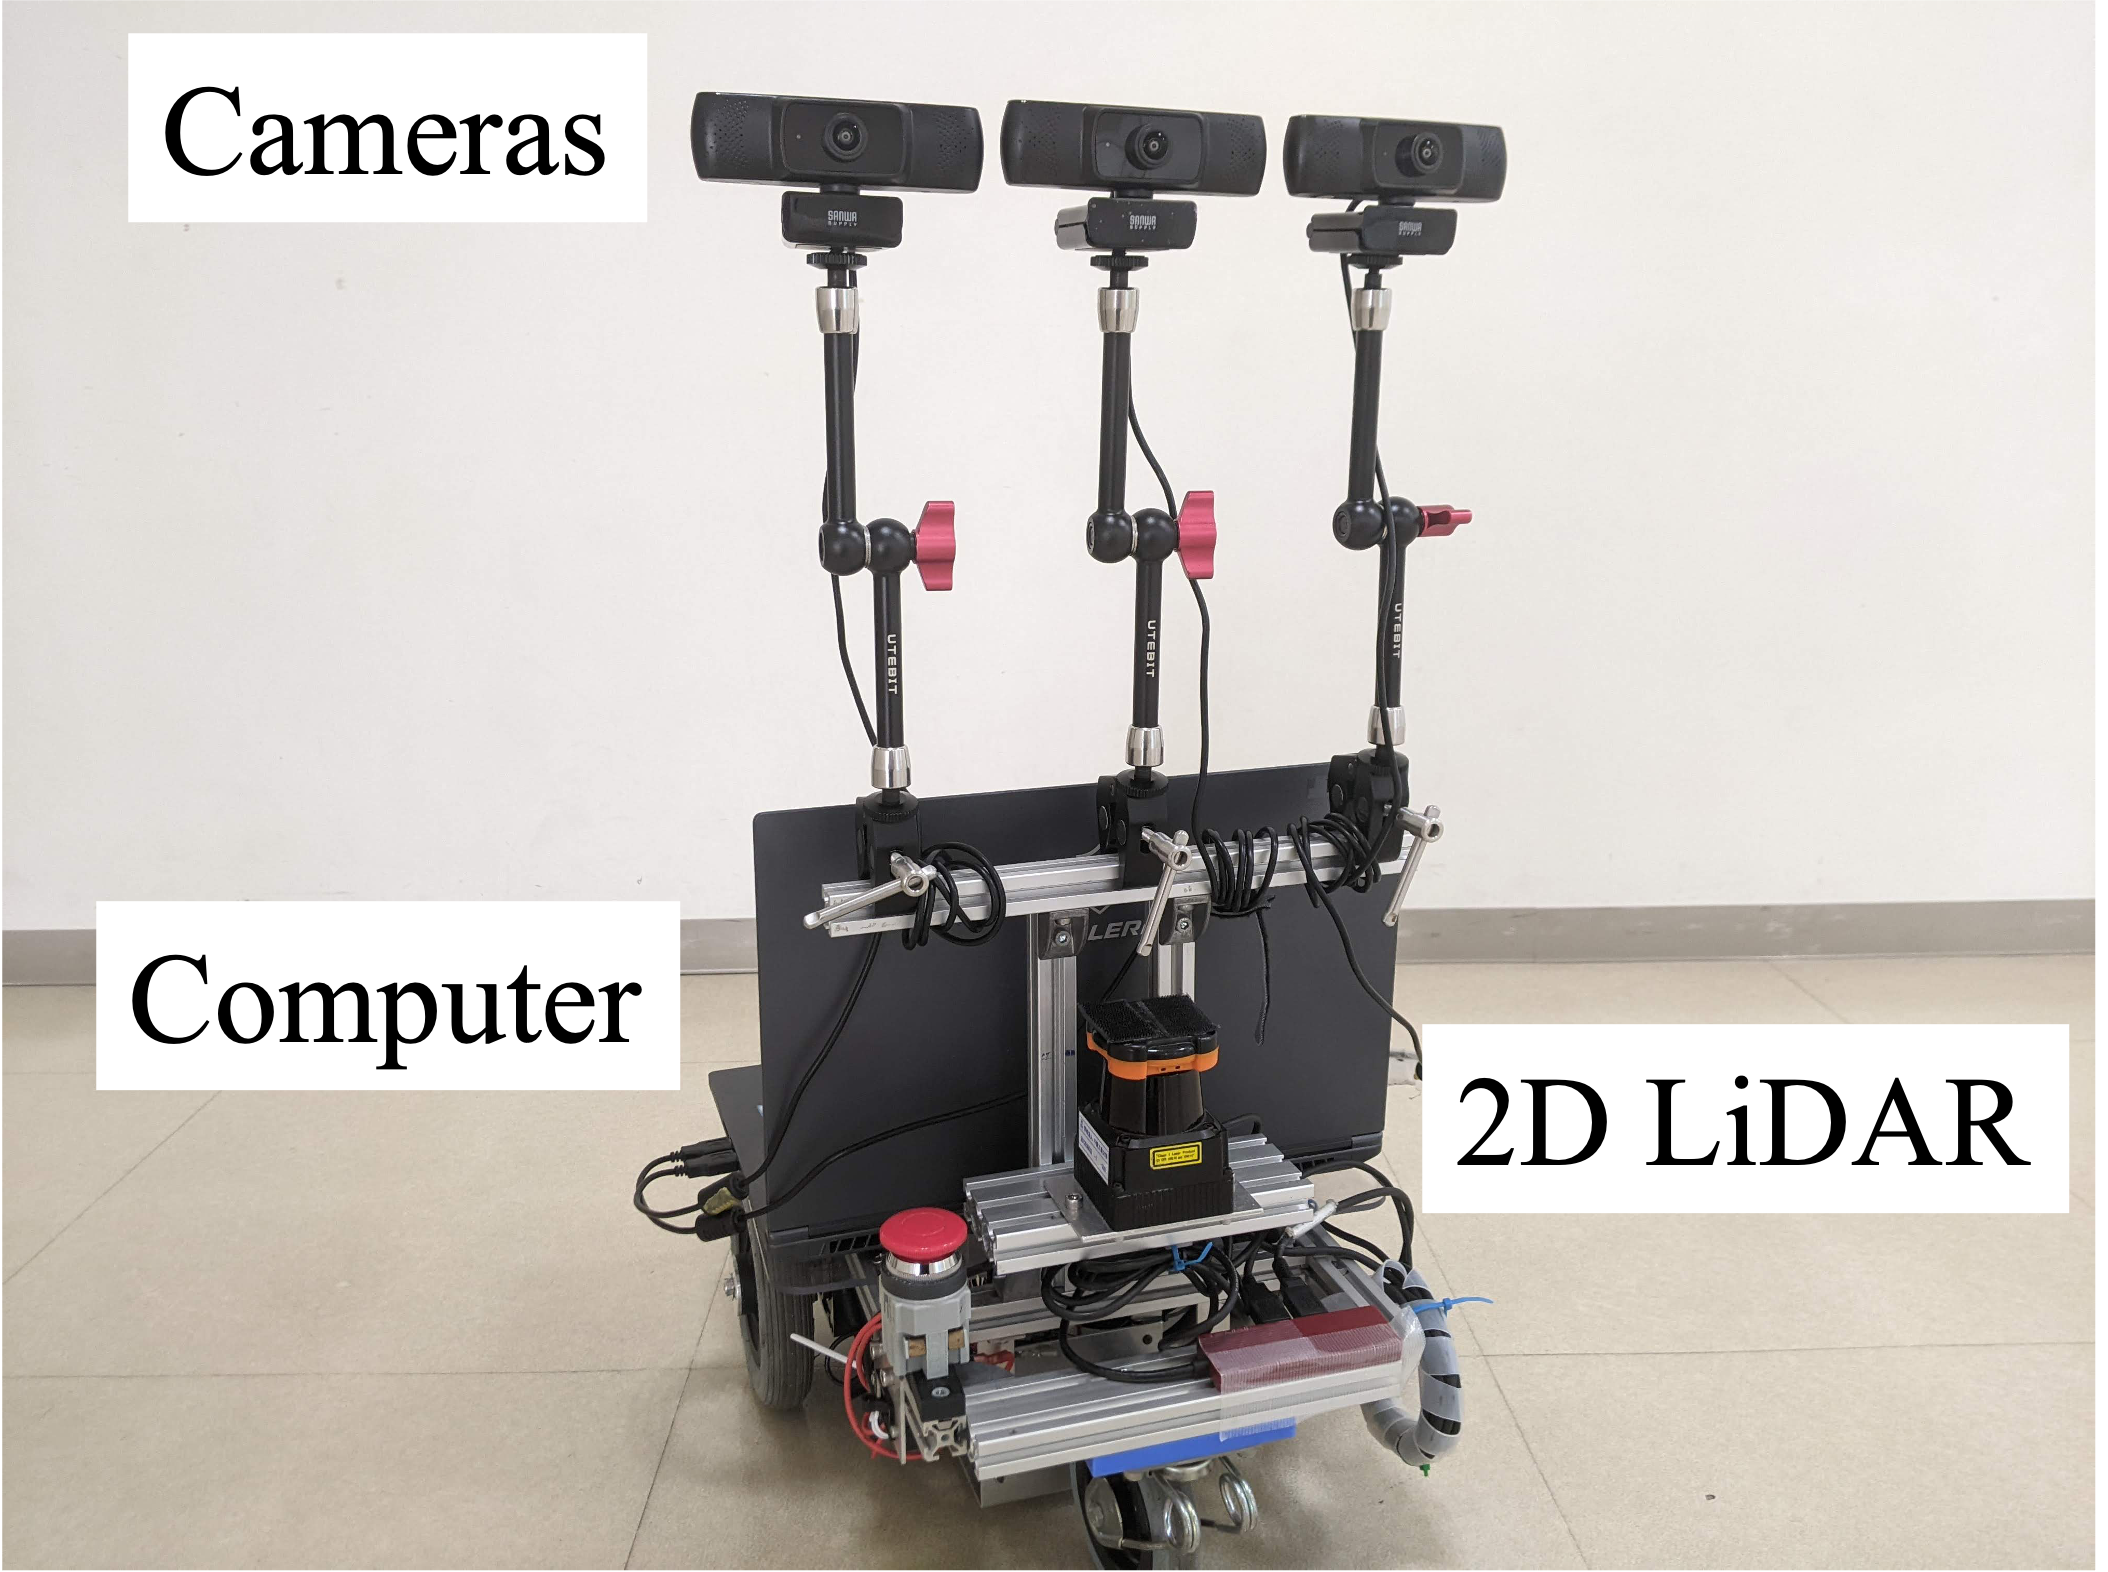
\includegraphics[height=40mm]{./figs/gamma_sensor.png}
     \caption{Experimental setup}\label{fig:gamma}
\end{figure}
\subsection{実験方法}
実験環境としてFig.\ref{fig:cit3f}で示した千葉工業大学津田沼キャンパス2号館3階の廊下を用いる.
% [藤原]と比較すると,突き当りが追加され,
% CとDが2つのこと行動を取ることが可能な分岐路へ変化している.
% 経路[藤原]で用いたa~fに図=で示したc~を追加した,a~nの順で走行する
% 前報と比較すると,突き当り,2つの行動がとれる分岐路C,Dが追加されている.
経路追従モジュールの訓練および通路分類器のデータセット収集ではFig.\ref{fig:newroute}で示した
aからnの経路を順番に走行する.
実験では島田らが用いた50例のシナリオの中から,
7例を用いた.選定の基準は,Fig.\ref{fig:cit3f}の場所を対象としていること.
ロボットが移動困難な狭い通路が含まれていないこと.
「後ろを向く」など経路追従モジュールができない行動が含まれていないことである.
% Fig.\ref{fig:cit3f}に示したエリアを対象として抽出した7例を用いる.
% シナリオの抽出において,1.地図を用いたルールベース制御器で通行が困難な場所が含まれるもの.
% 2.その場で「右を向く」といった経路追従モジュールが達成困難なもの
% を除外している.\par
まずはじめに通路分類器の訓練を行う.
前述の経路を地図に基づいたルールベース制御器の出力を用いて,3周し,
データセットを収集する.
% その際,データセットへのデータの追加は0.125秒周期で行う.
収集したデータは,1,2周目を訓練データとし,3周目をテストデータとする.
それぞれのデータ数は,
訓練データ5781,テストデータ2902である.
訓練はバッチサイズを32として,30epoch行った.
訓練の結果,テストデータに対するAccuracyは0.98であった.\par
次に経路追従モジュールの訓練を行う.
通路分類器の訓練と同様の経路を,オンラインで模倣学習しながら1周走行する.
その際のステップ数は12000であった.
% データセットへのデータの追加は0.2秒周期で行う.
\par
2つのモジュールを訓練後,1例のシナリオをシステムに入力する.
この入力したシナリオのスタート地点へロボットを配置し,目的地までの自律移動を開始する.
% なお,経路から外れるといった要因で走行の継続が困難になった場合でも即時失敗とせず,
% 失敗箇所を記録しながら,人間が介入し,実験を継続する.
Fig.\ref{fig:scenario_exp}に実験で用いた7例のシナリオを示す.
% 今回は,実験環境を2号館3階の一部のエリアに限定しているが,
% 今後はフロア全体へ拡張する予定である.
\begin{figure}[htbp]
    \centering
     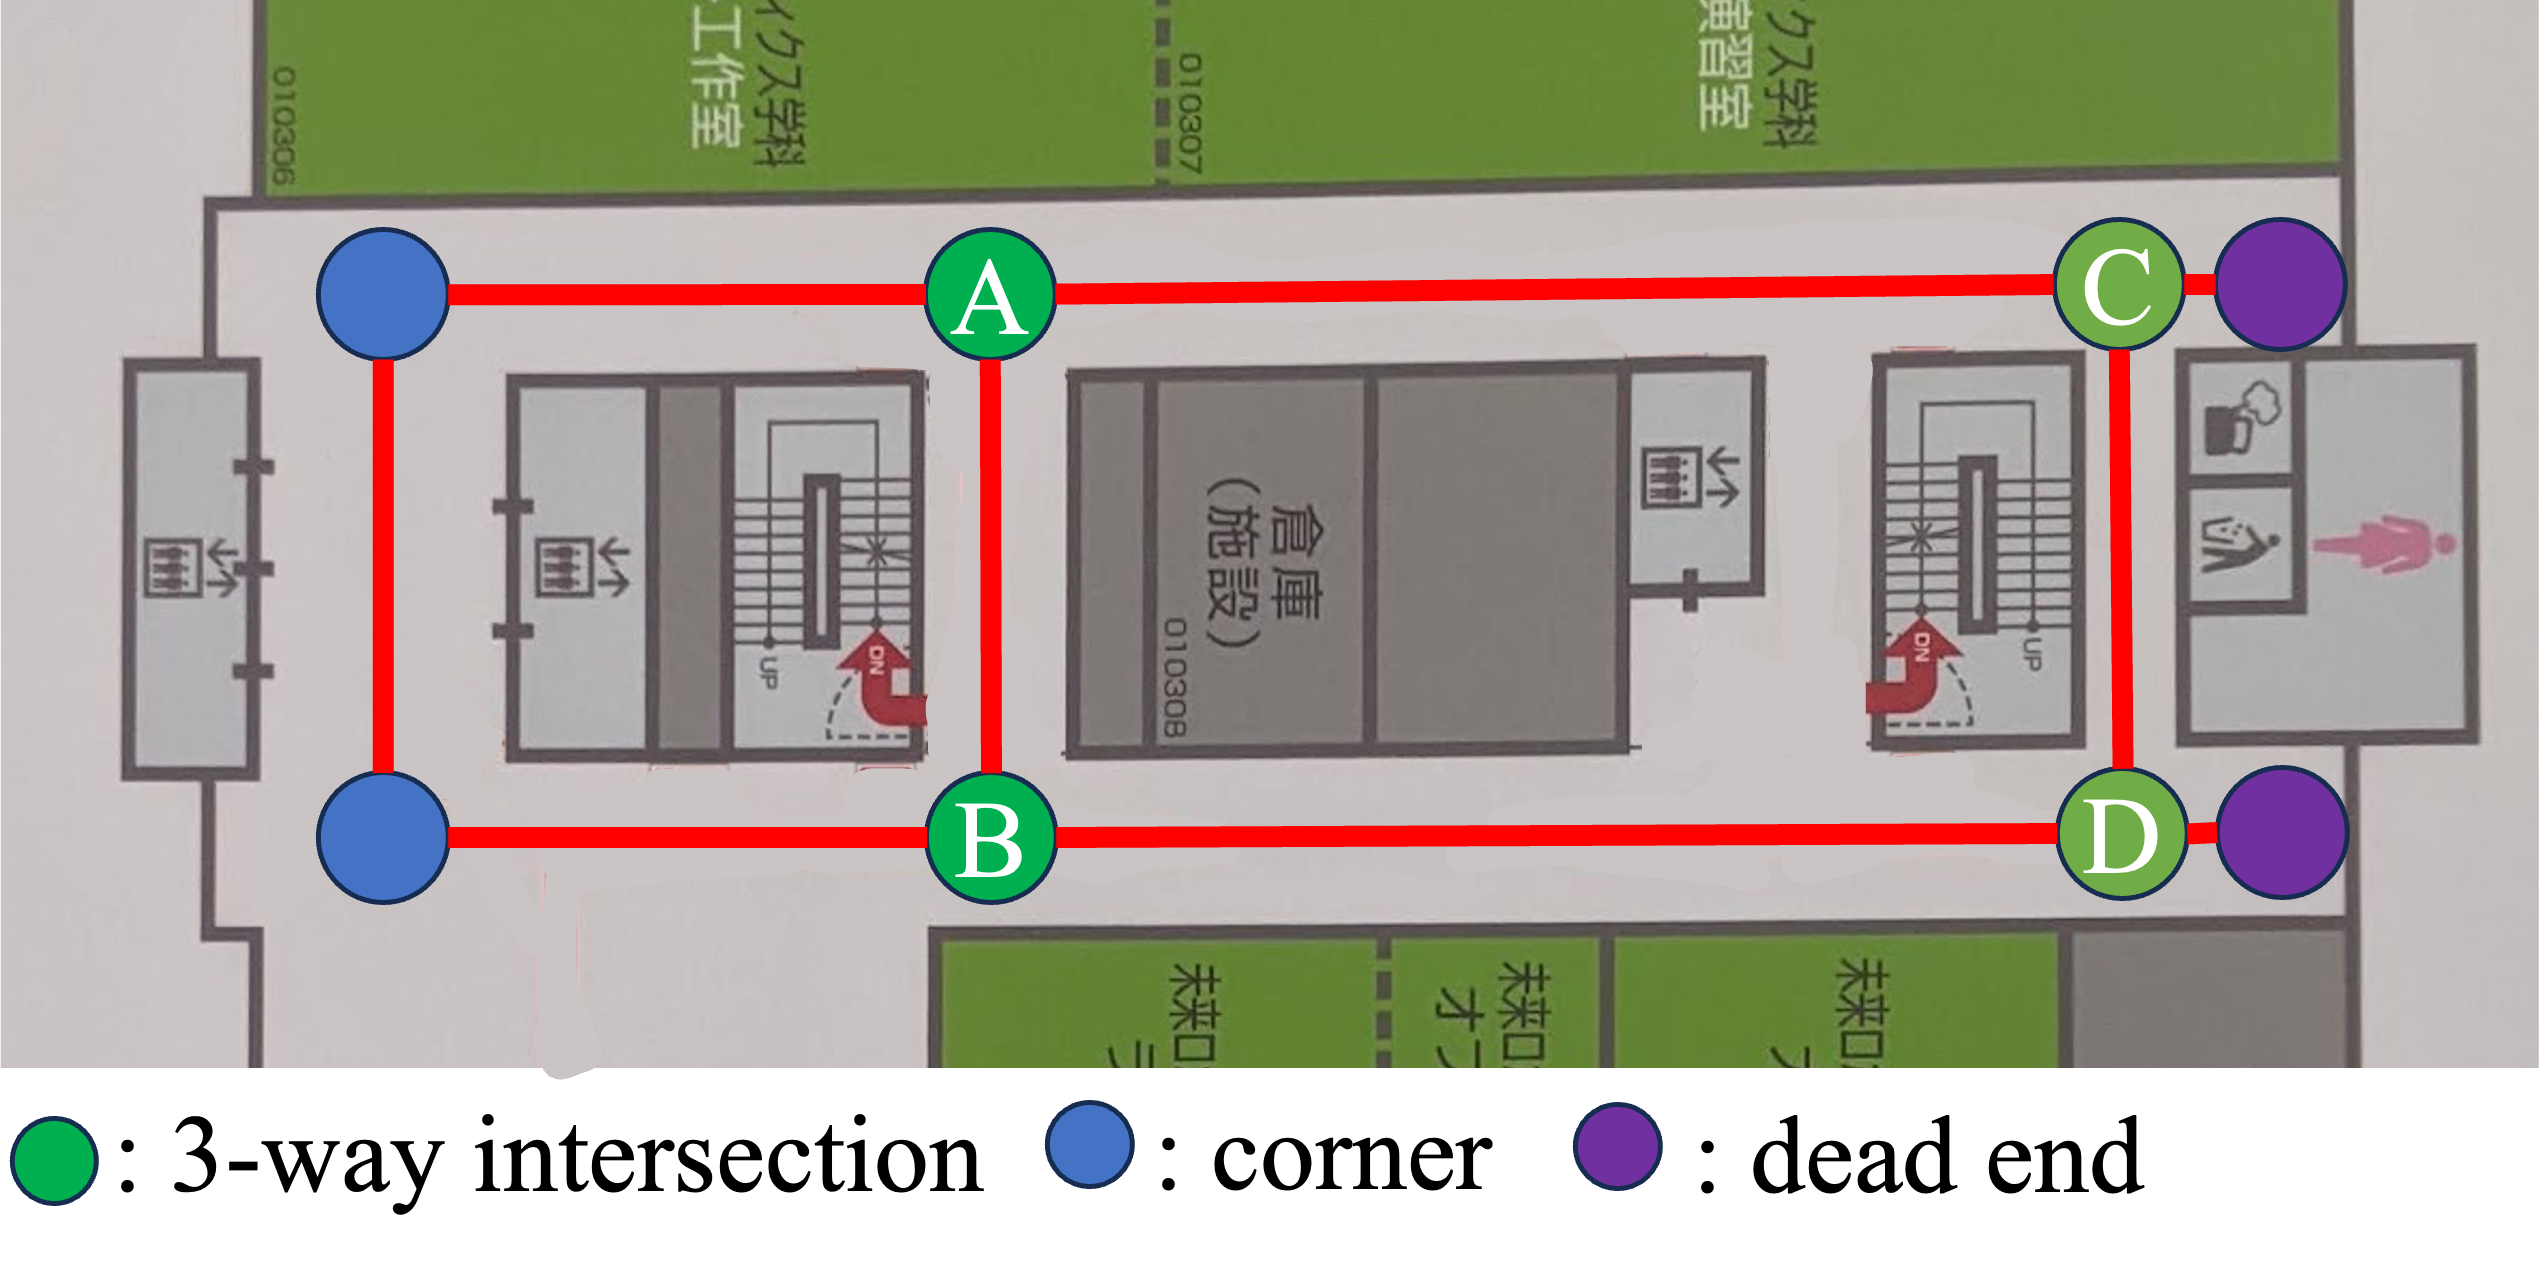
\includegraphics[height=40mm,width=80mm]{./figs/cit3f.png}
     \caption{Experimental environment}\label{fig:cit3f}
\end{figure}
% \begin{figure}[htbp]
%     \centering
%      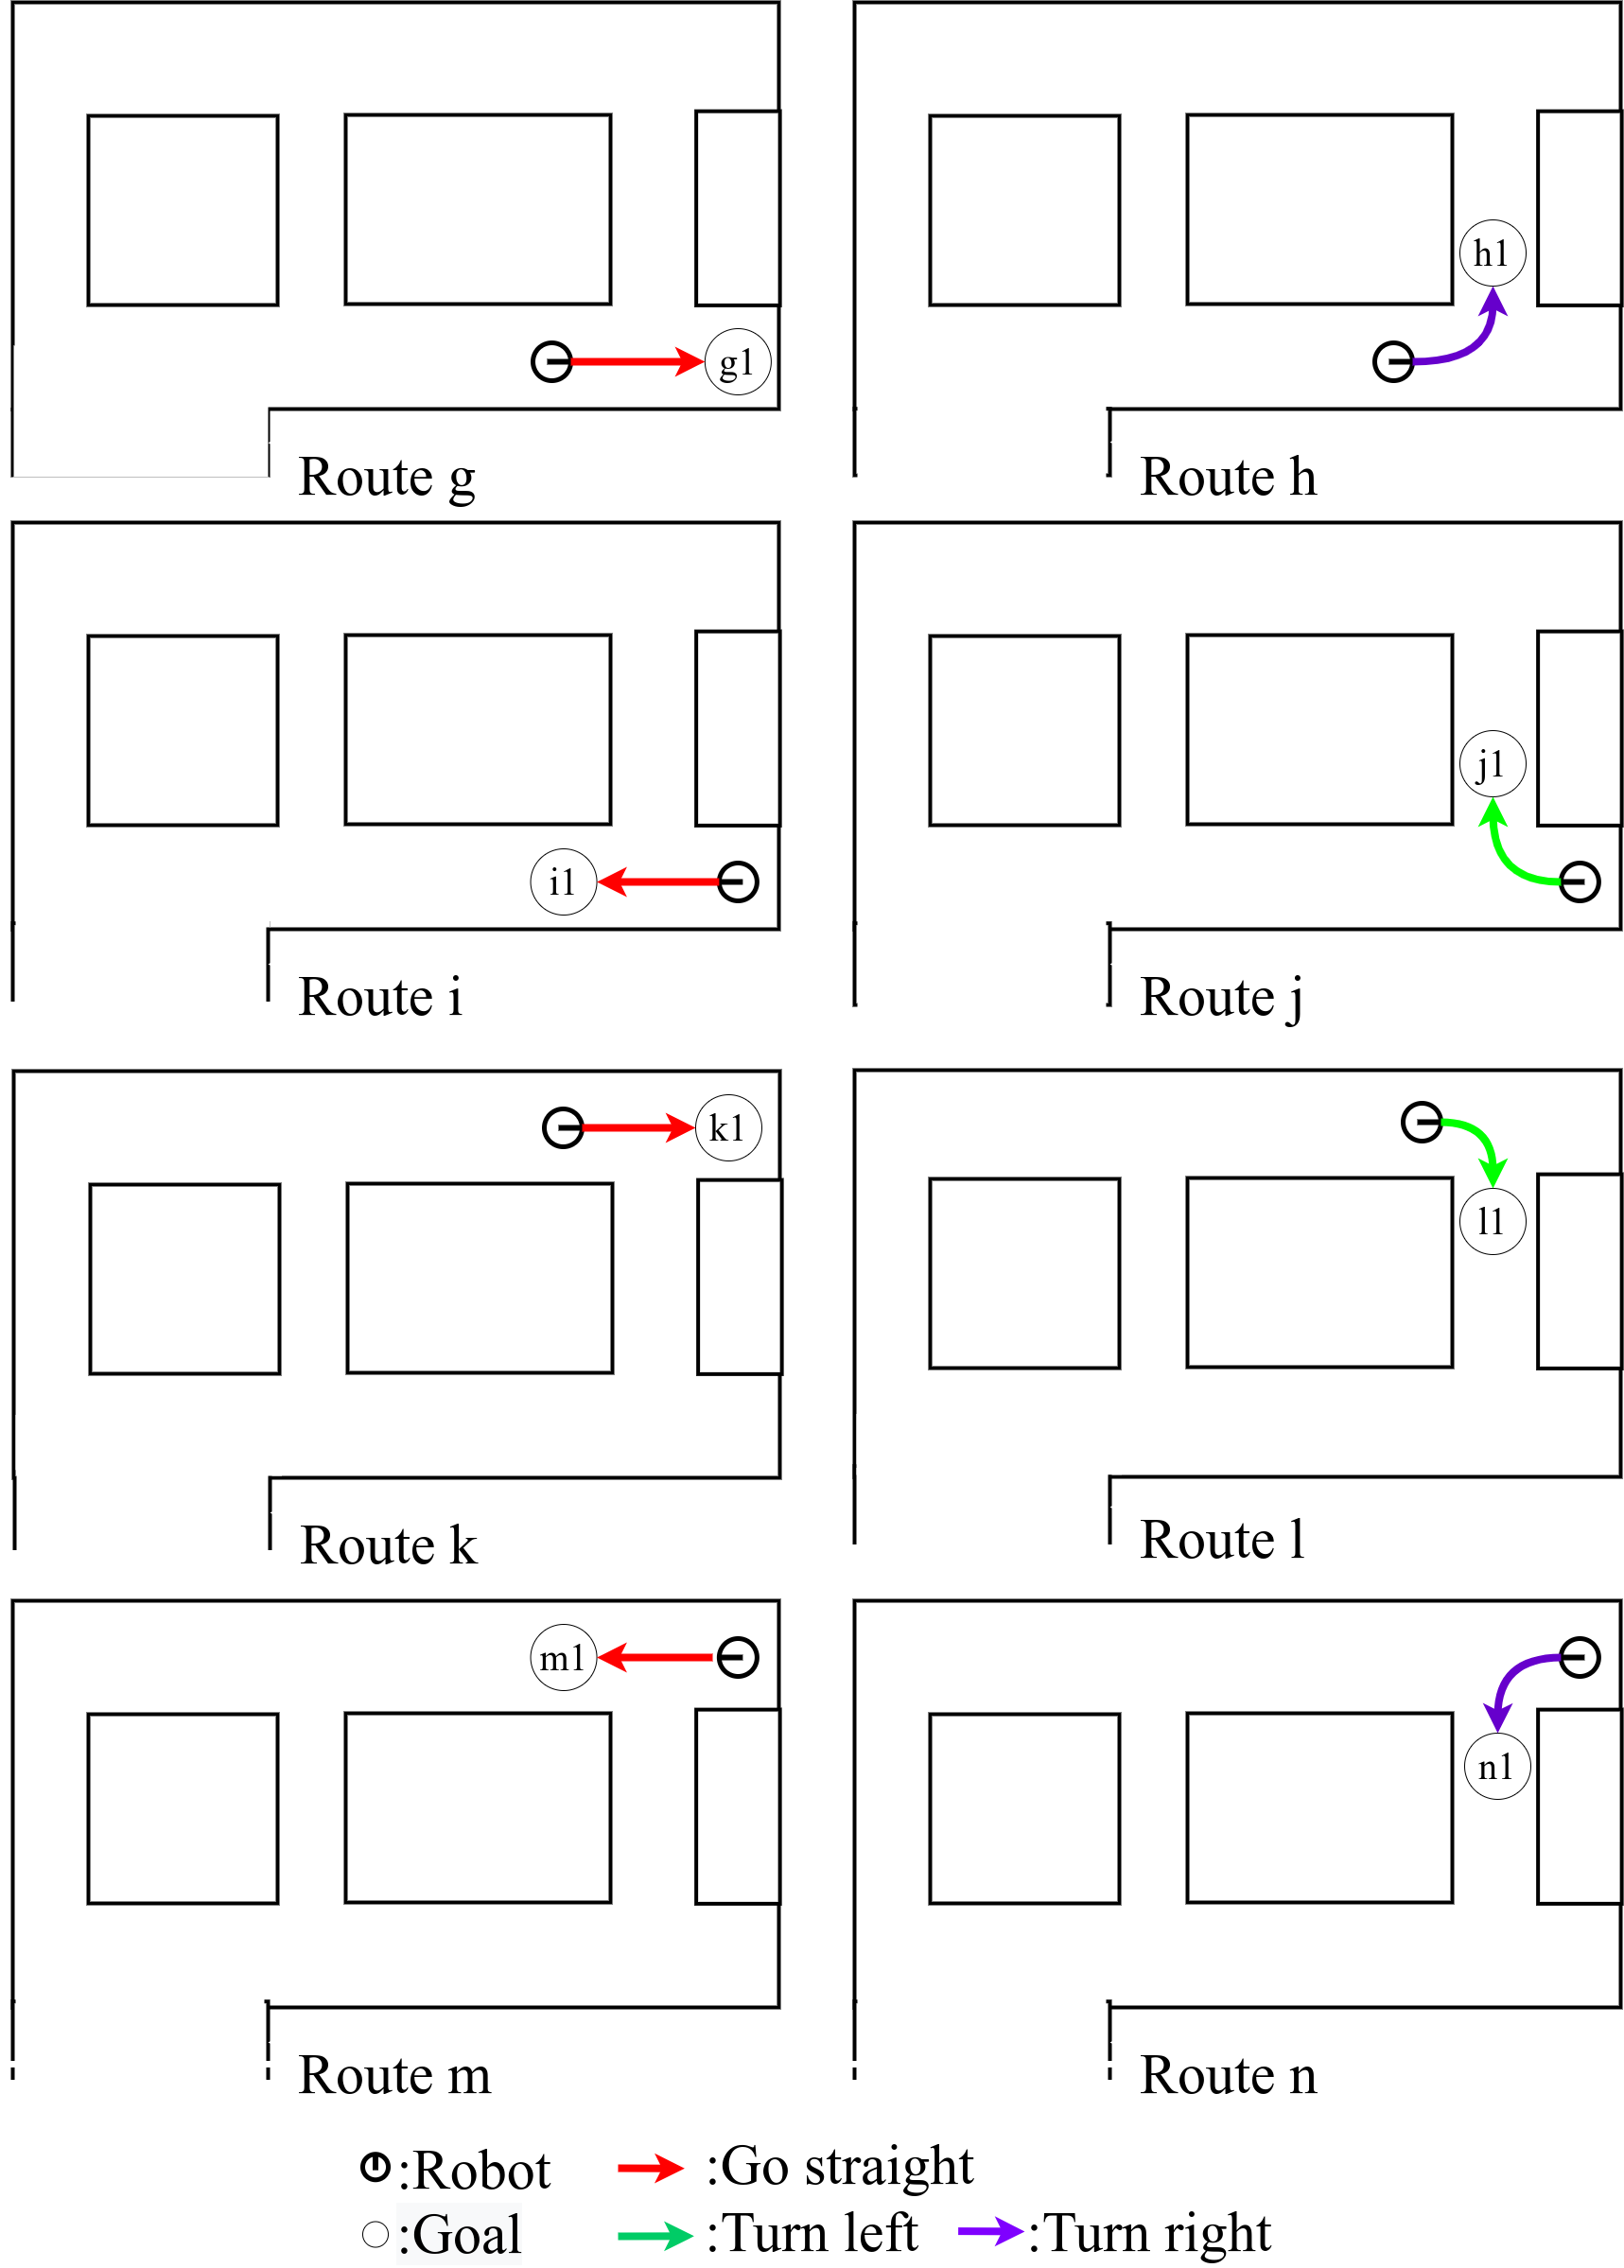
\includegraphics[height=100mm,width=80mm]{./figs/newroute.png}
%      \caption{Route for the added experiment}\label{fig:newroute}
% \end{figure}

% \begin{figure}[h!]
%     \centering
%      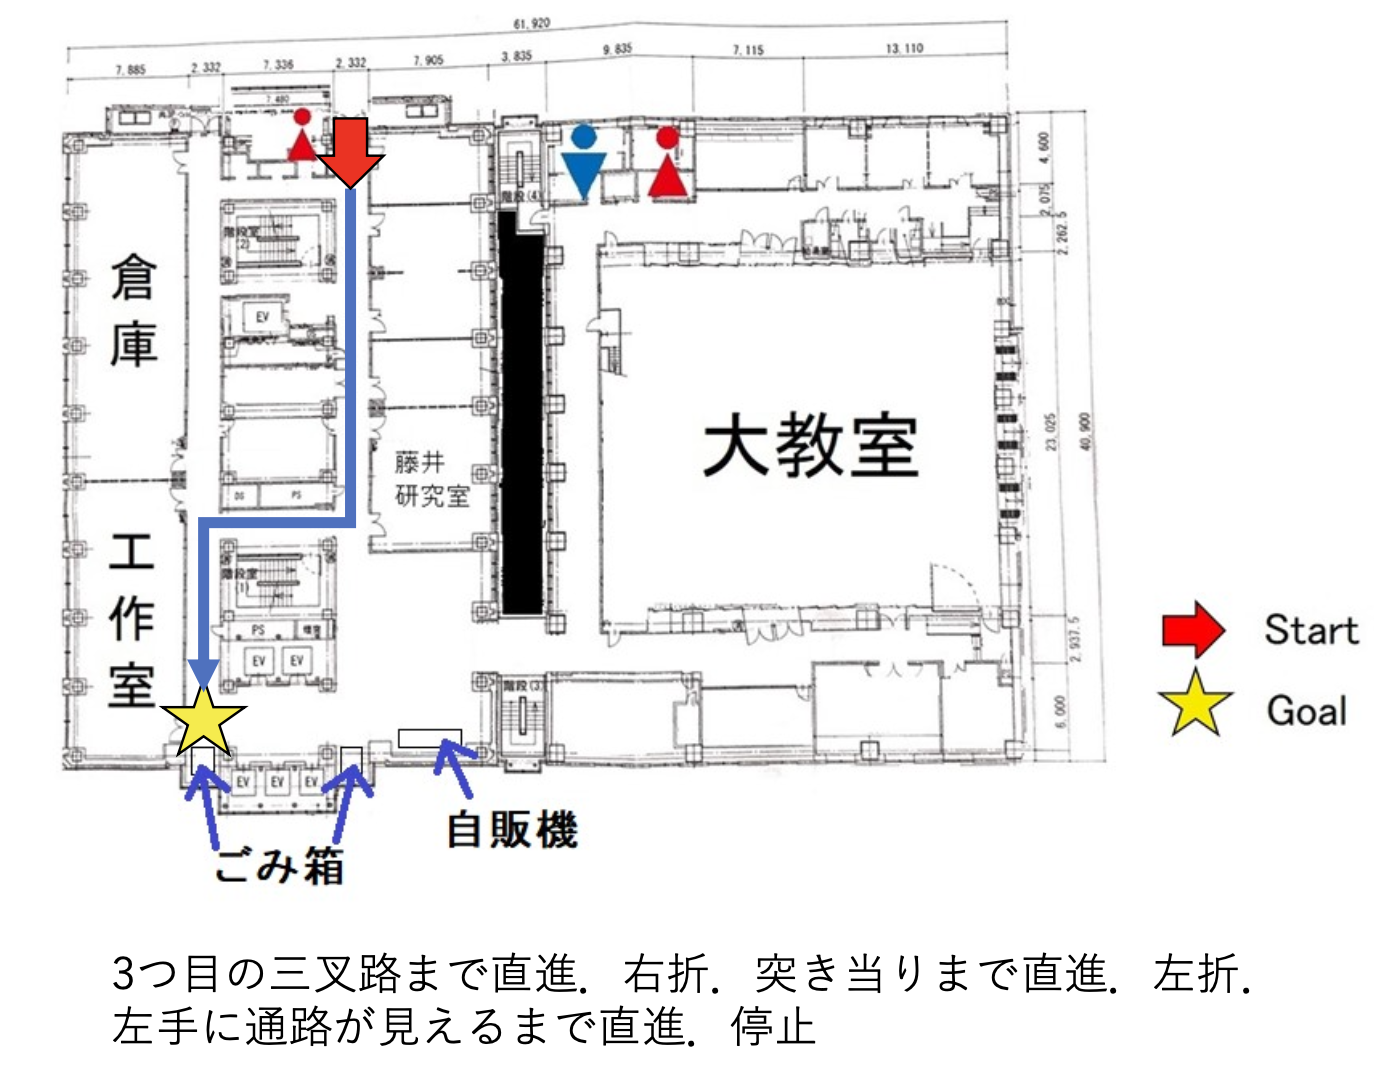
\includegraphics[height=50mm]{./figs/scenario24.png}
%      \caption{Example of the scenario}\label{fig:scenario24}
% \end{figure}
% \begin{figure}[htbp]\vspace*{-2zh}


\subsection{実験結果}
% 実験結果をTable \ref{tab:result}に示す.
% 表はそれぞれ実験に用いたシナリオの番号,学習器の出力が要因による介入の回数,
% 通路分類の間違いを要因とする介入の回数である.
Fig.\ref{fig:exp_path}にFig.\ref{fig:scenario24}における経路追従の様子を示す.
結果として,7例すべての例でロボットが,
指定された経路を追従して目的地へ到達した.
以上の結果から,提案するカメラ画像とシナリオに基づいて,
経路を追従して目的地まで自律移動する手法の有効性が確認された.
% シナリオに基づくナビゲーションとカメラ画像による通路分類を追加したシステムが,
% 適切に動作することを確認した.


\section{結言}
本稿では,事前に作成したメトリックマップを用いず,カメラ画像とシナリオに基づいて
経路を追従して目的地まで自律移動する手法を提案した.
そして,実ロボットを用いた実験により提案手法の有効性を検証した.
% 経路選択機能を持つ学習器を用いた走行に対して,
% カメラ画像からの目標方向の生成を目的として,シナリオを
% 用いたナビゲーションと通路分類器の
% 追加を行った.
% 実験では,提案手法により,指示された経路を
% カメラ画像に基づいて,追従し,目的地へ到達なことを確認した
% 学習器がカメラ画像と生成された目標方向を用いて,
% 指定された経路に沿って目的地へ到達可能なことを確認した.
% 今後は,実験環境をより広い屋内,または屋外へと拡大する予定である.
% \begin{figure}[htbp]
%     \centering
%      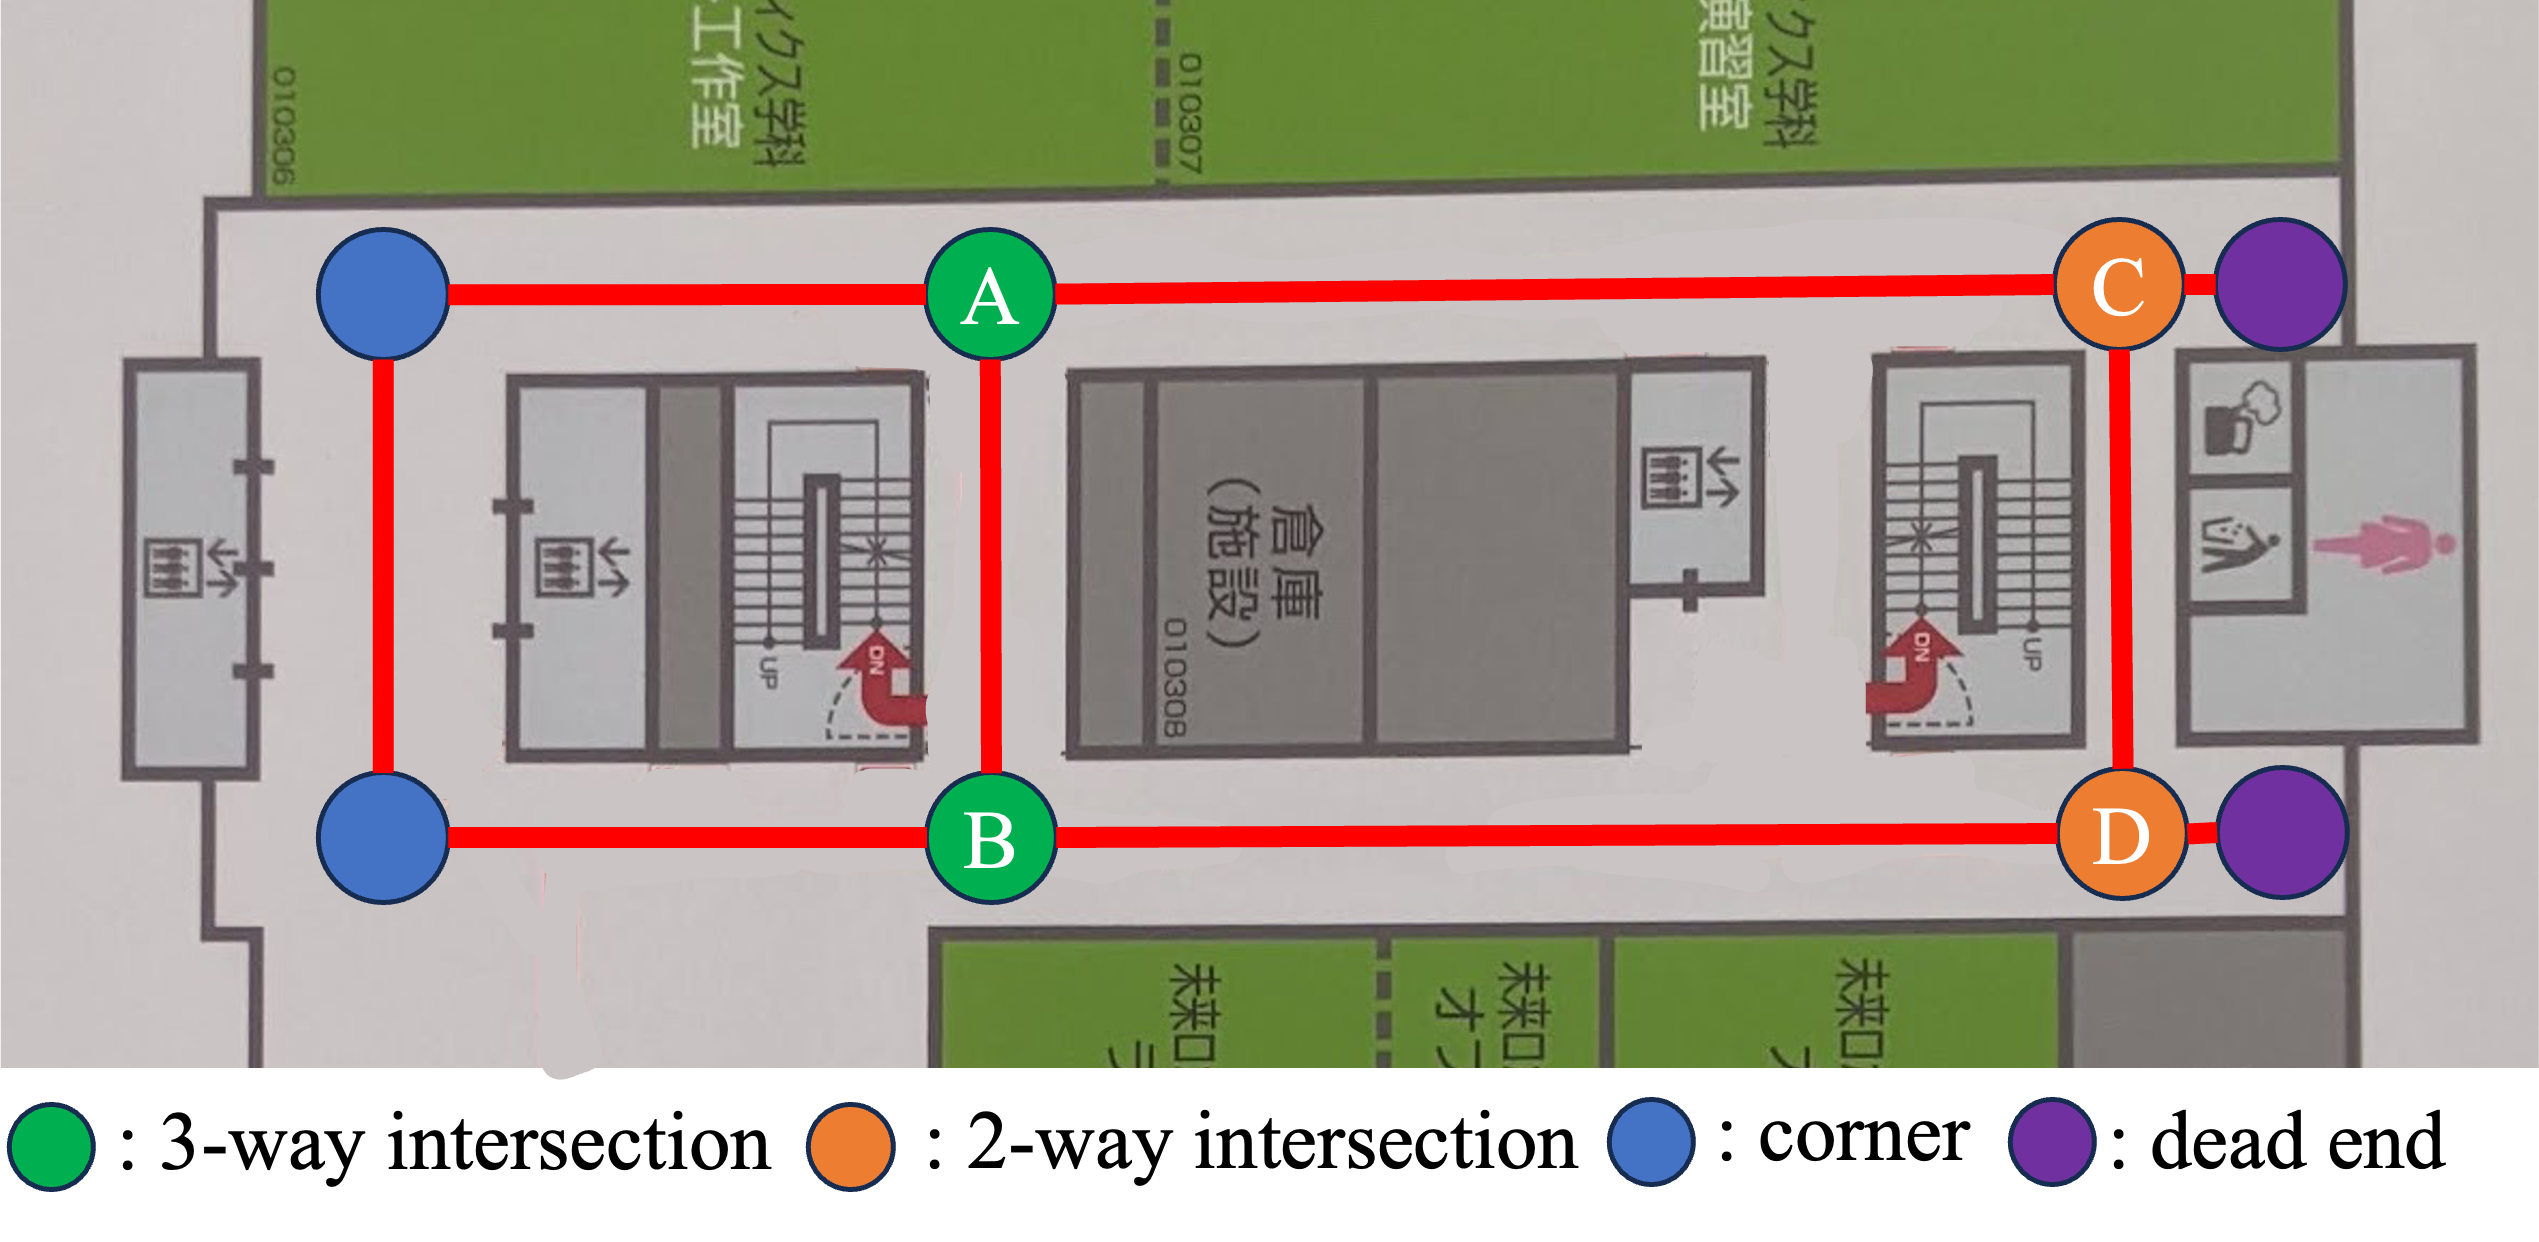
\includegraphics[height=40mm,width=80mm]{./figs/keiro.png}
%      \caption{Experimental environment}\label{fig:cit3f}
% \end{figure}

\printbibliography[title=参考文献]
\begin{figure*}[t]
    \centering
     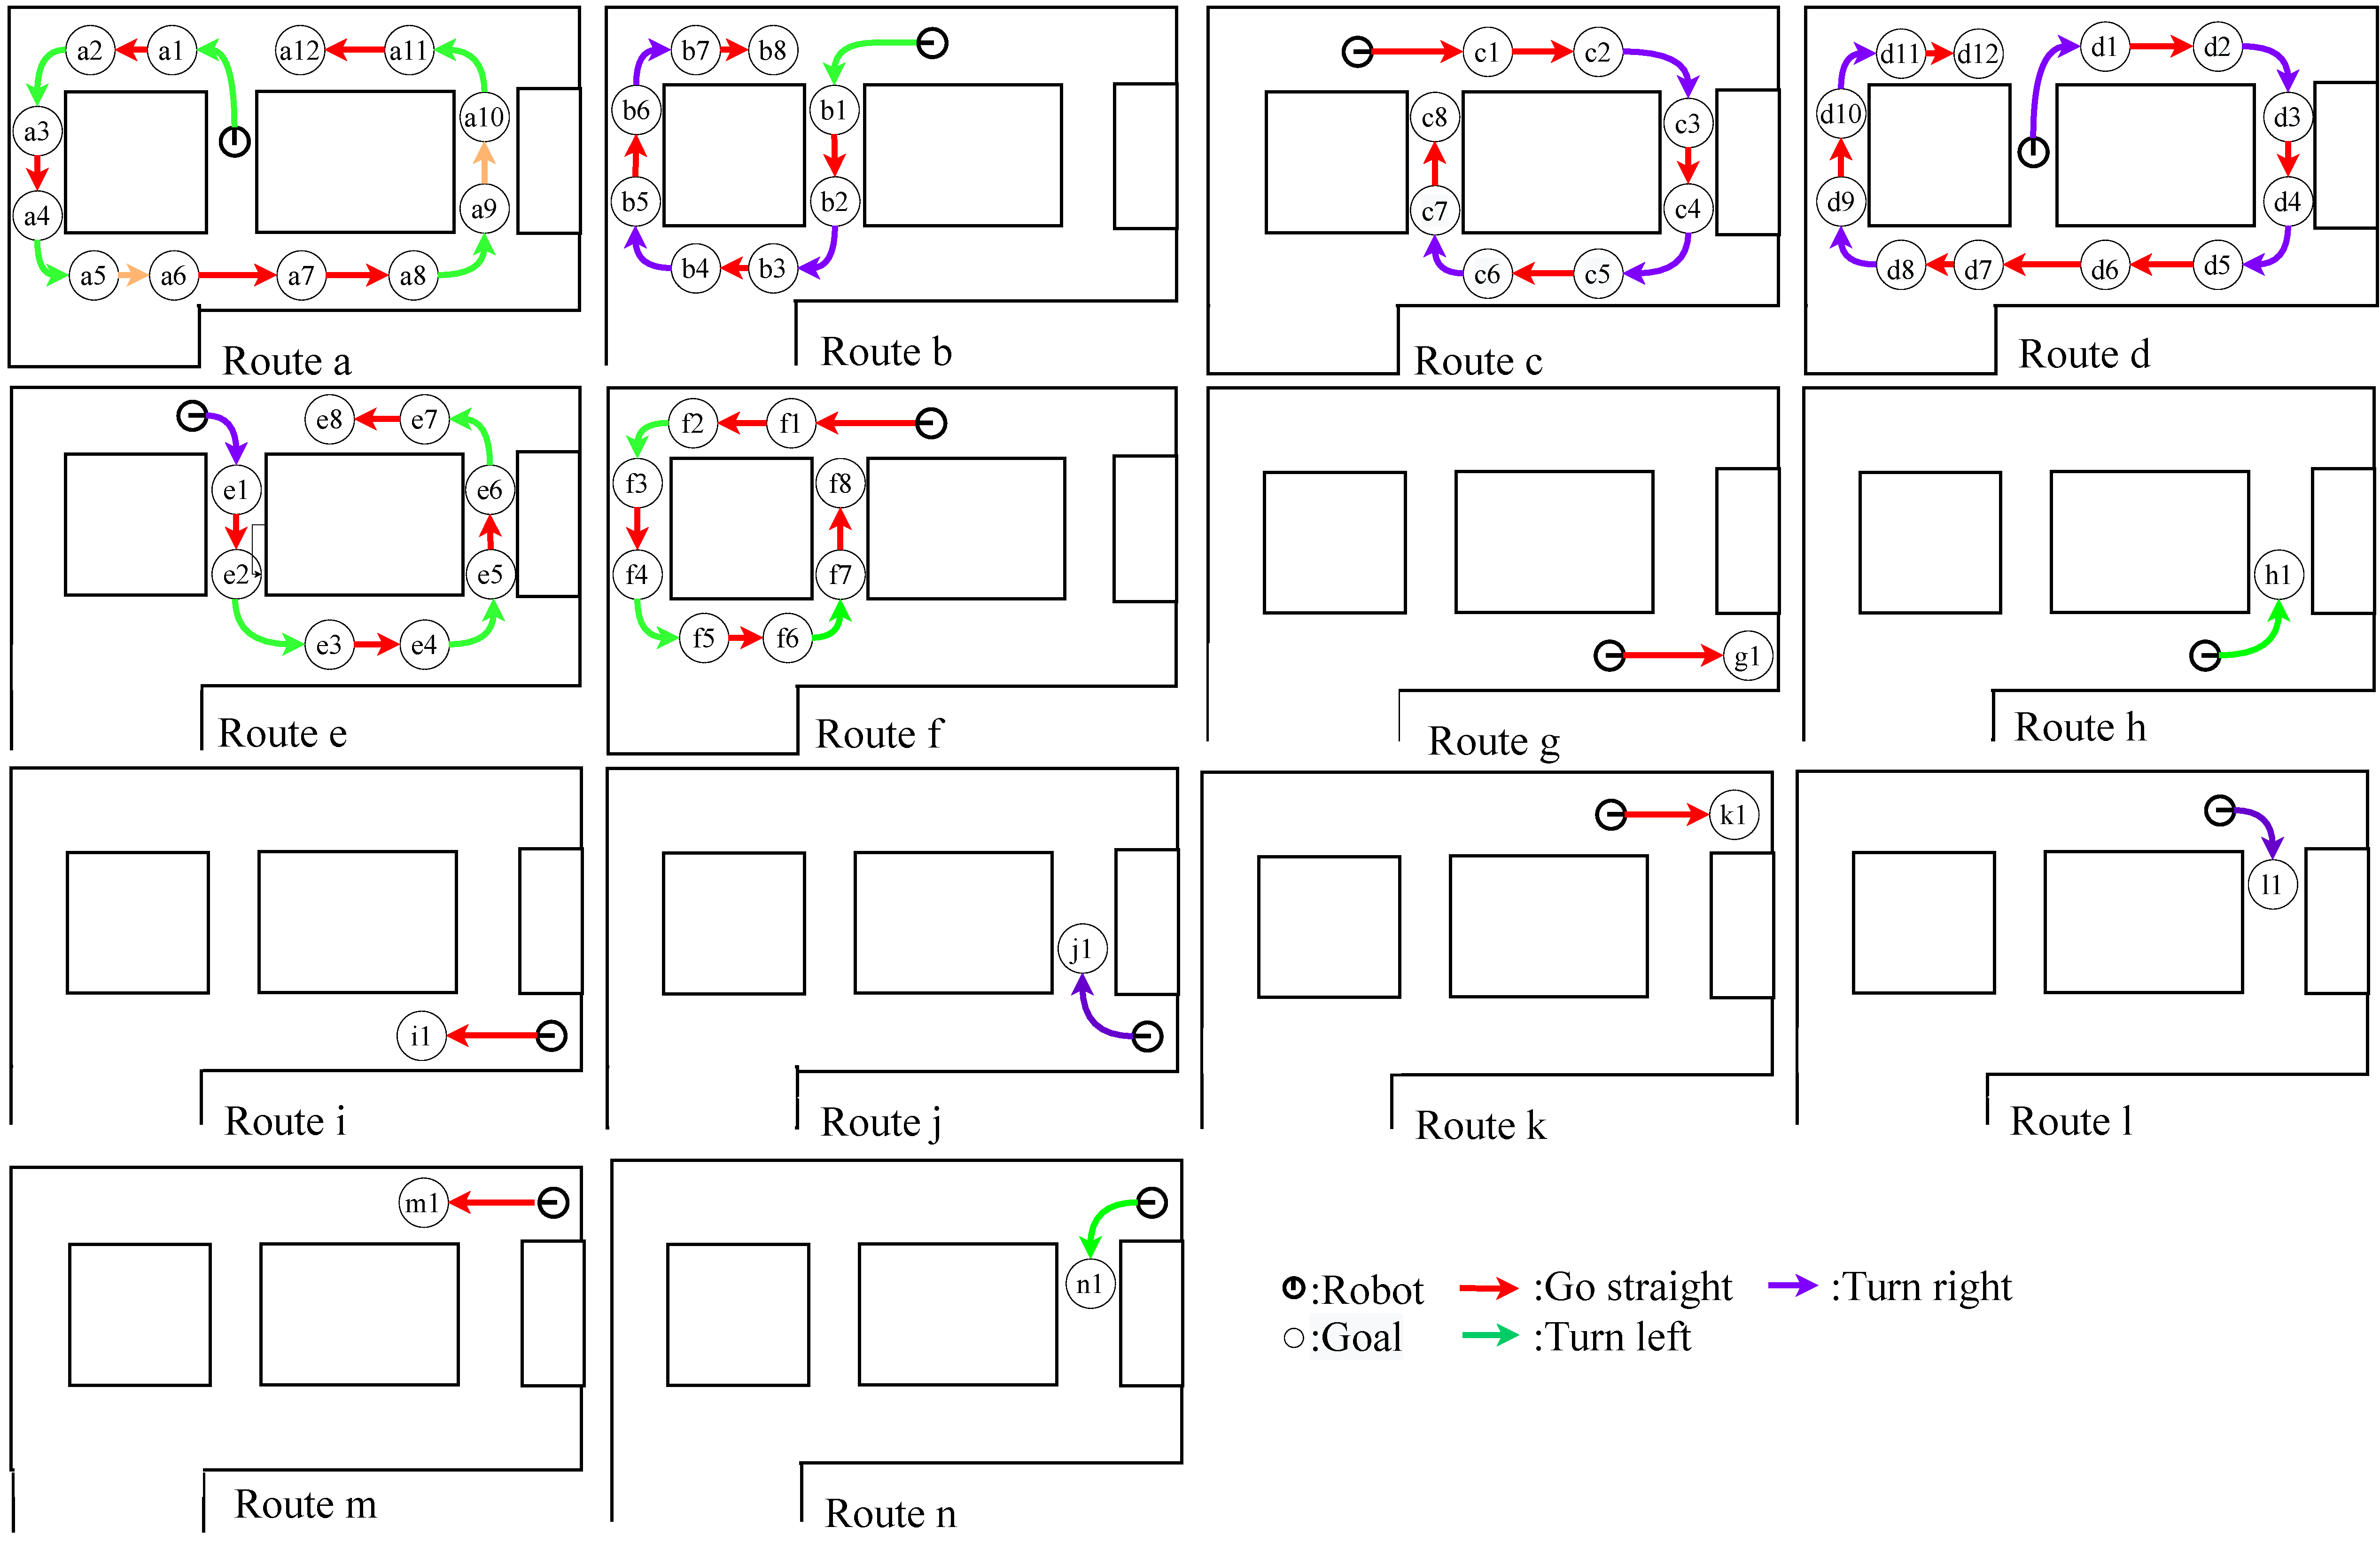
\includegraphics[height=120mm,width=160mm]{./figs/newroute.pdf}
     \caption{Route used for learning}\label{fig:newroute}
\end{figure*}

\setlength\textfloatsep{0pt}
\begin{figure*}[t]
    \begin{tabular}{ccc}
        \begin{minipage}[t]{0.3\textwidth}
            \centering
            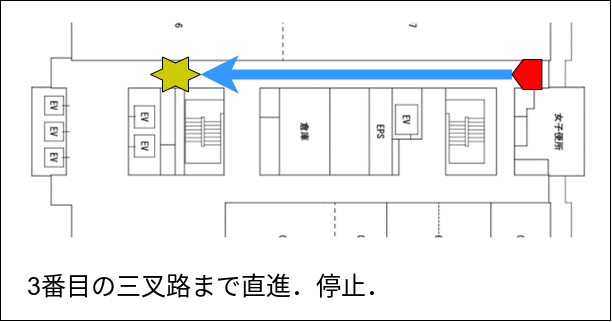
\includegraphics[keepaspectratio, width=55mm]{figs/scenario/scenario01.png}
            \subcaption{Scenario 01}
            \label{composite}
        \end{minipage} &
        \begin{minipage}[t]{0.3\textwidth}
            \centering
            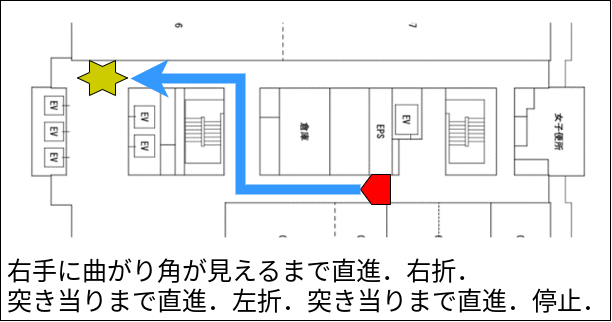
\includegraphics[keepaspectratio, width=55mm]{figs/scenario/scenario02.png}
            \subcaption{Scenario 02}
            \label{Gradation}
        \end{minipage} &
        \begin{minipage}[t]{0.3\textwidth}
            \centering
            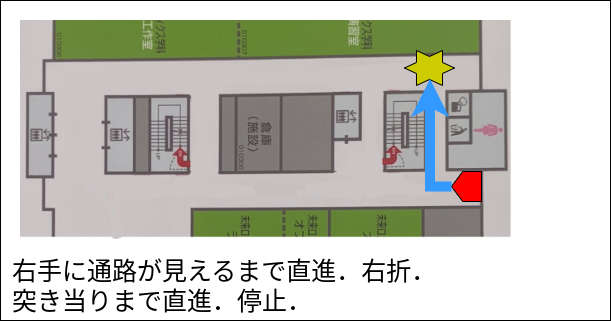
\includegraphics[keepaspectratio, width=55mm]{figs/scenario/scenario03.png}
            \subcaption{Scenario 03}
            \label{fill}
        \end{minipage} \\
        \begin{minipage}[t]{0.3\textwidth}
            \centering
            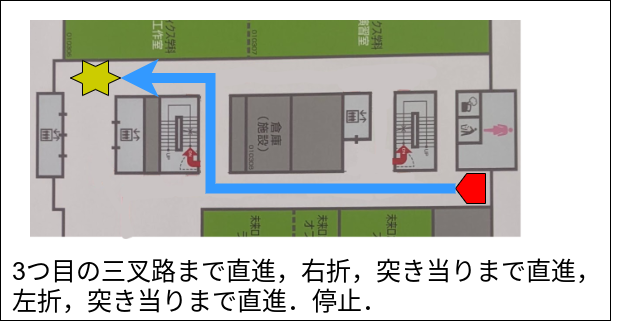
\includegraphics[keepaspectratio, width=55mm]{figs/scenario/scenario04.png}
            \subcaption{Scenario 04}
            \label{transform}
        \end{minipage} &
        \begin{minipage}[t]{0.3\textwidth}
            \centering
            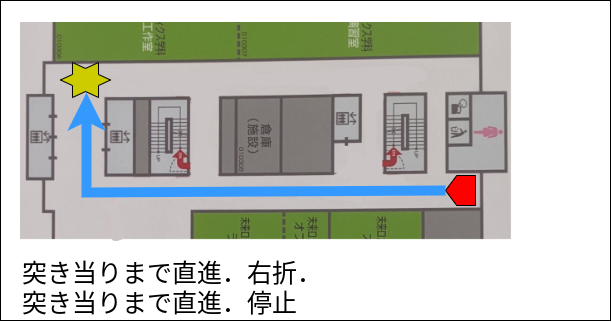
\includegraphics[keepaspectratio, width=55mm]{figs/scenario/scenario05.png}
            \subcaption{Scenario 05}
            \label{image1}
        \end{minipage} &
        \begin{minipage}[t]{0.3\textwidth}
            \centering
            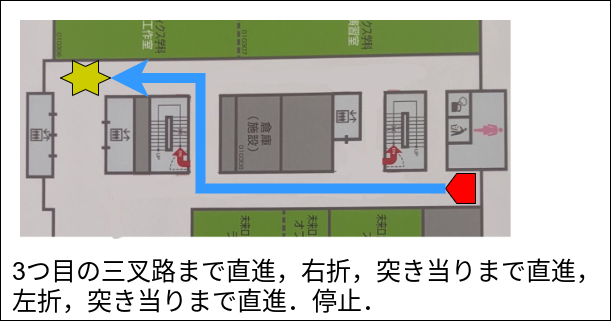
\includegraphics[keepaspectratio, width=55mm]{figs/scenario/scenario06.png}
            \subcaption{Scenario 06}
            \label{fig:scenario24}
        \end{minipage}\\
        \begin{minipage}[t]{0.3\textwidth}
            \centering
            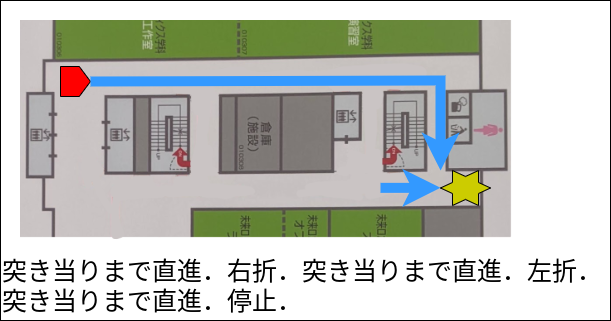
\includegraphics[keepaspectratio, width=55mm]{figs/scenario/scenario07.png}
            \subcaption{Scenario 07}
            \label{imagess}
        \end{minipage}
    \end{tabular}
    \caption{Scenario used in the experiment}\label{fig:scenario_exp}
\end{figure*}

\begin{figure*}[t]\vspace*{-10zh}
    \begin{tabular}{ccc}
        \begin{minipage}[t]{0.5\textwidth}
            \centering
            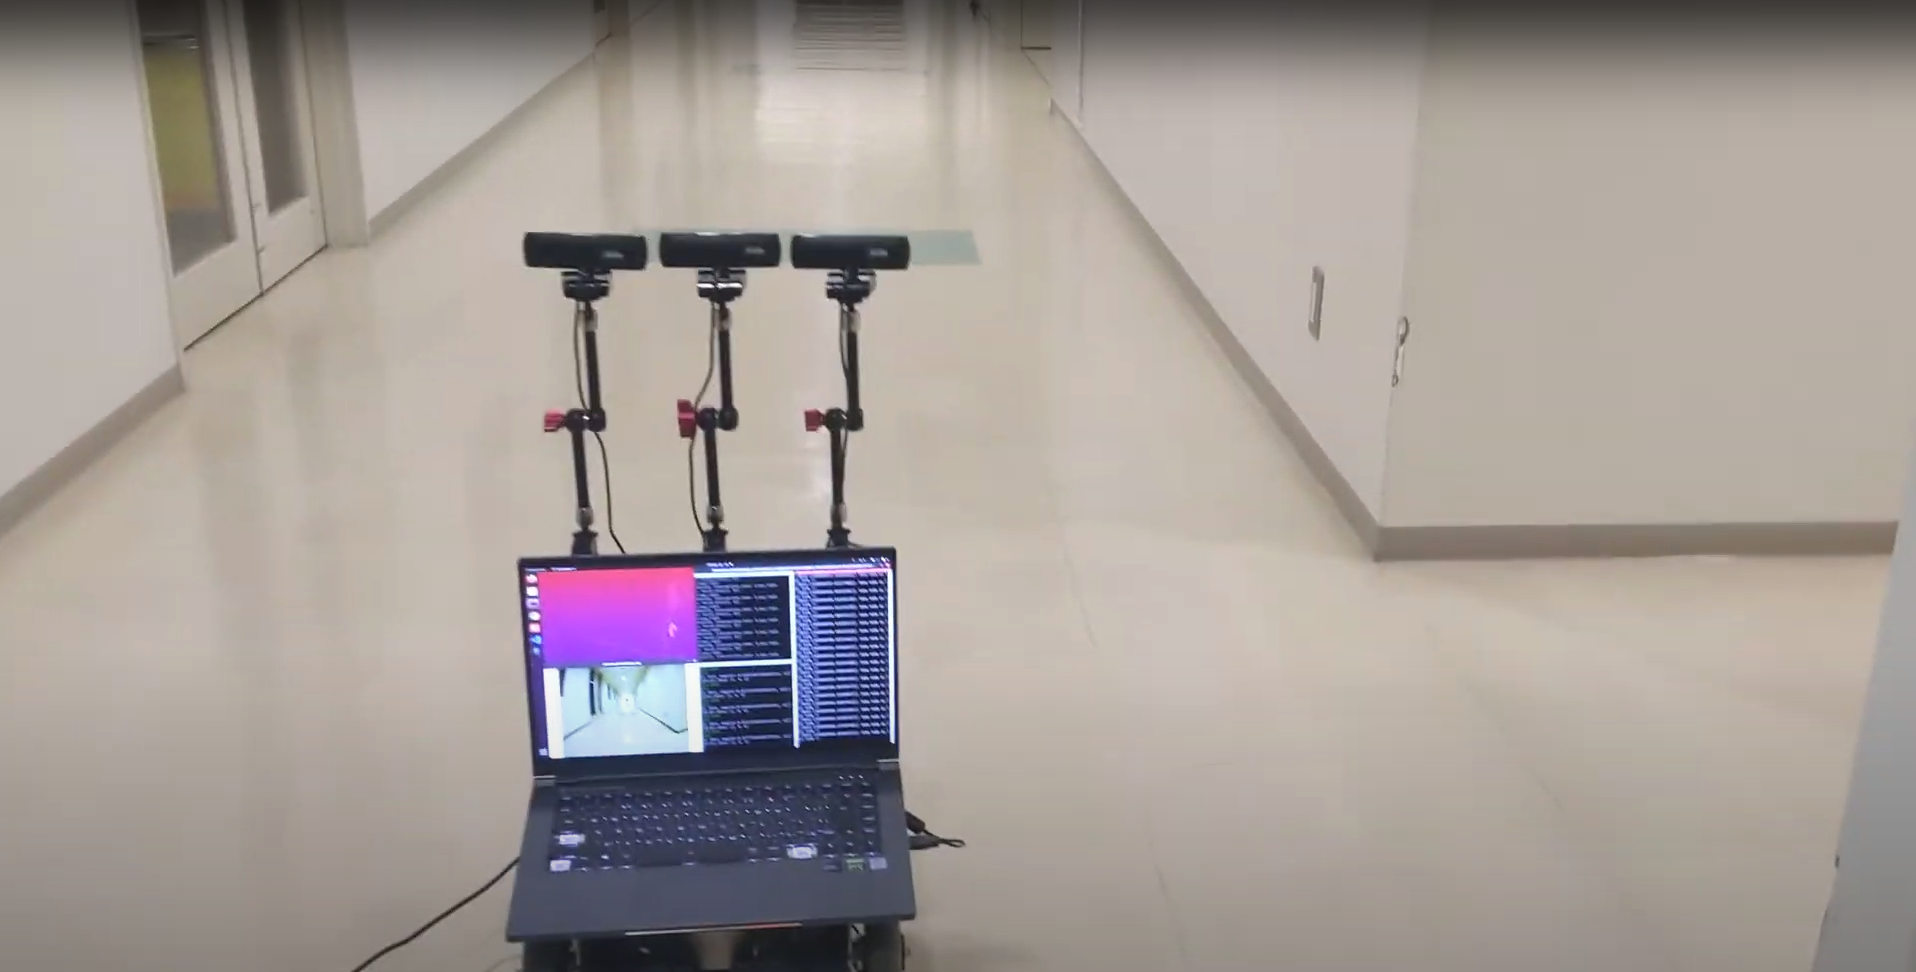
\includegraphics[keepaspectratio, width=80mm]{figs/exp_path_follow_0.png}
            \subcaption{3つ目の三叉路まで直進(First 3-way)}
        \end{minipage} &
        \begin{minipage}[t]{0.5\textwidth}
            \centering
            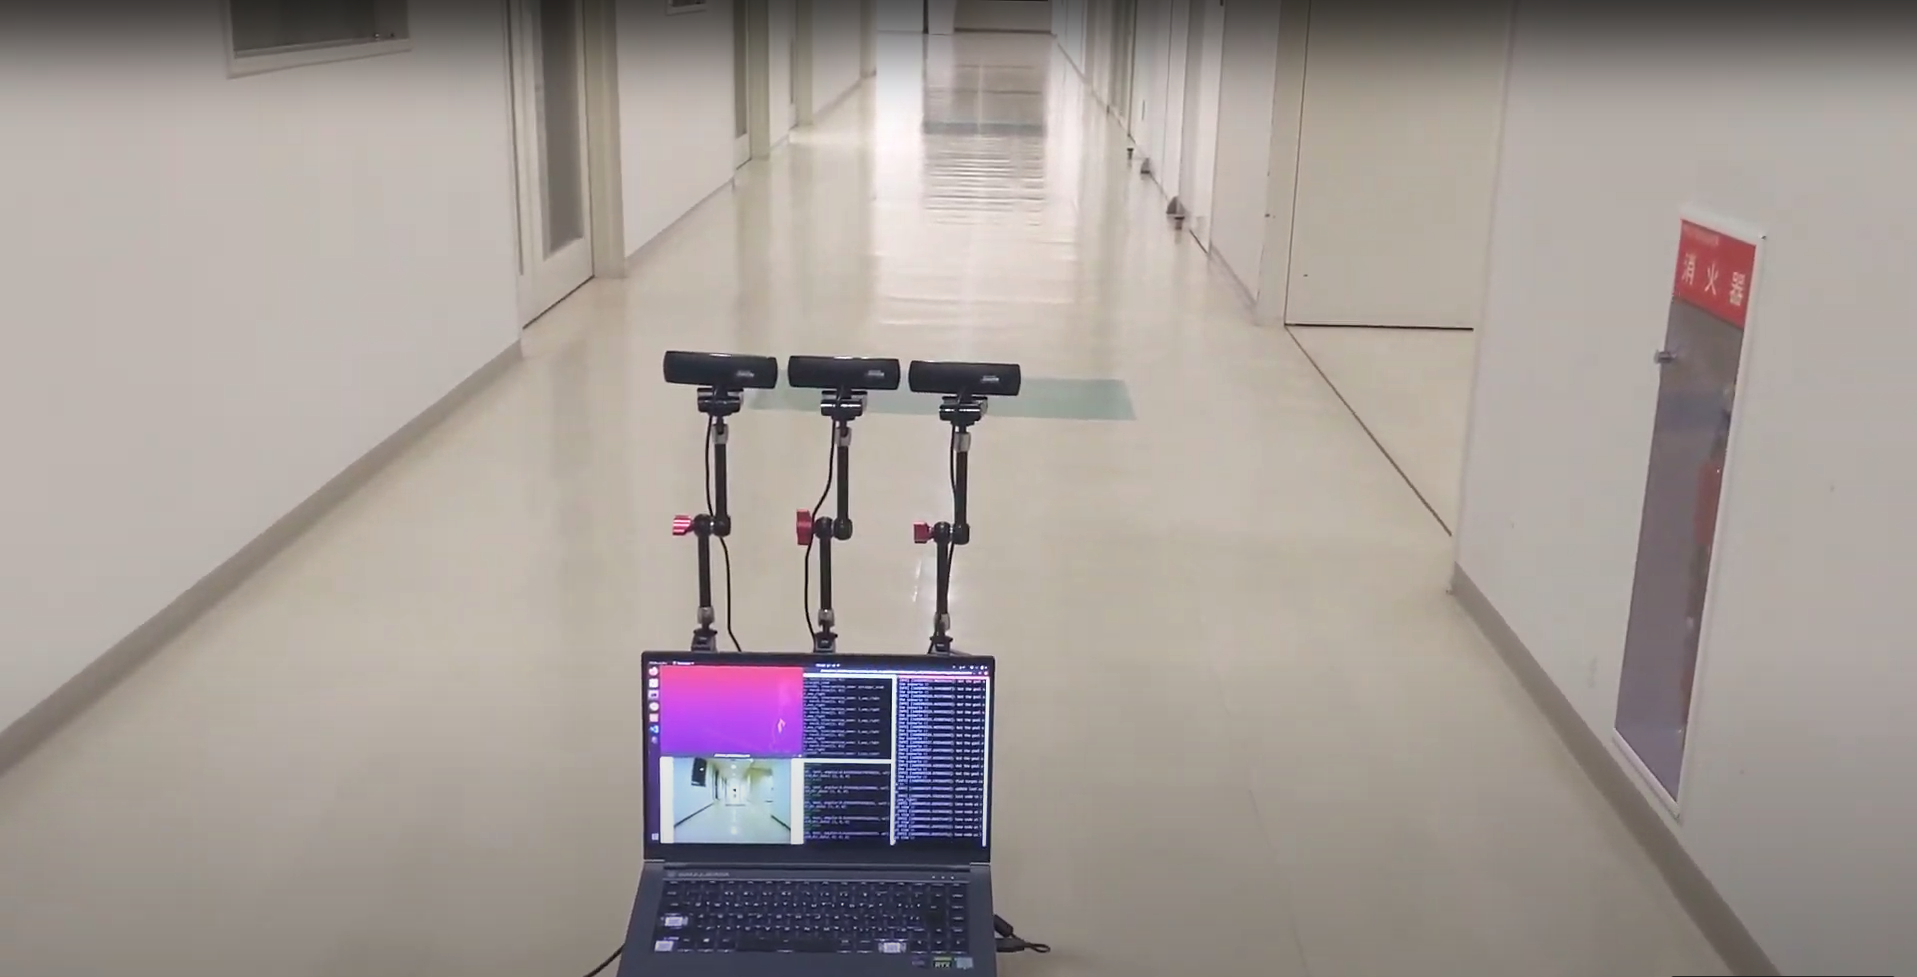
\includegraphics[keepaspectratio, width=80mm]{figs/exp_path_follow_1.png}
            \subcaption{3つ目の三叉路まで直進(Second 3-way)}
        \end{minipage} \\

        \begin{minipage}[t]{0.5\textwidth}
            \centering
            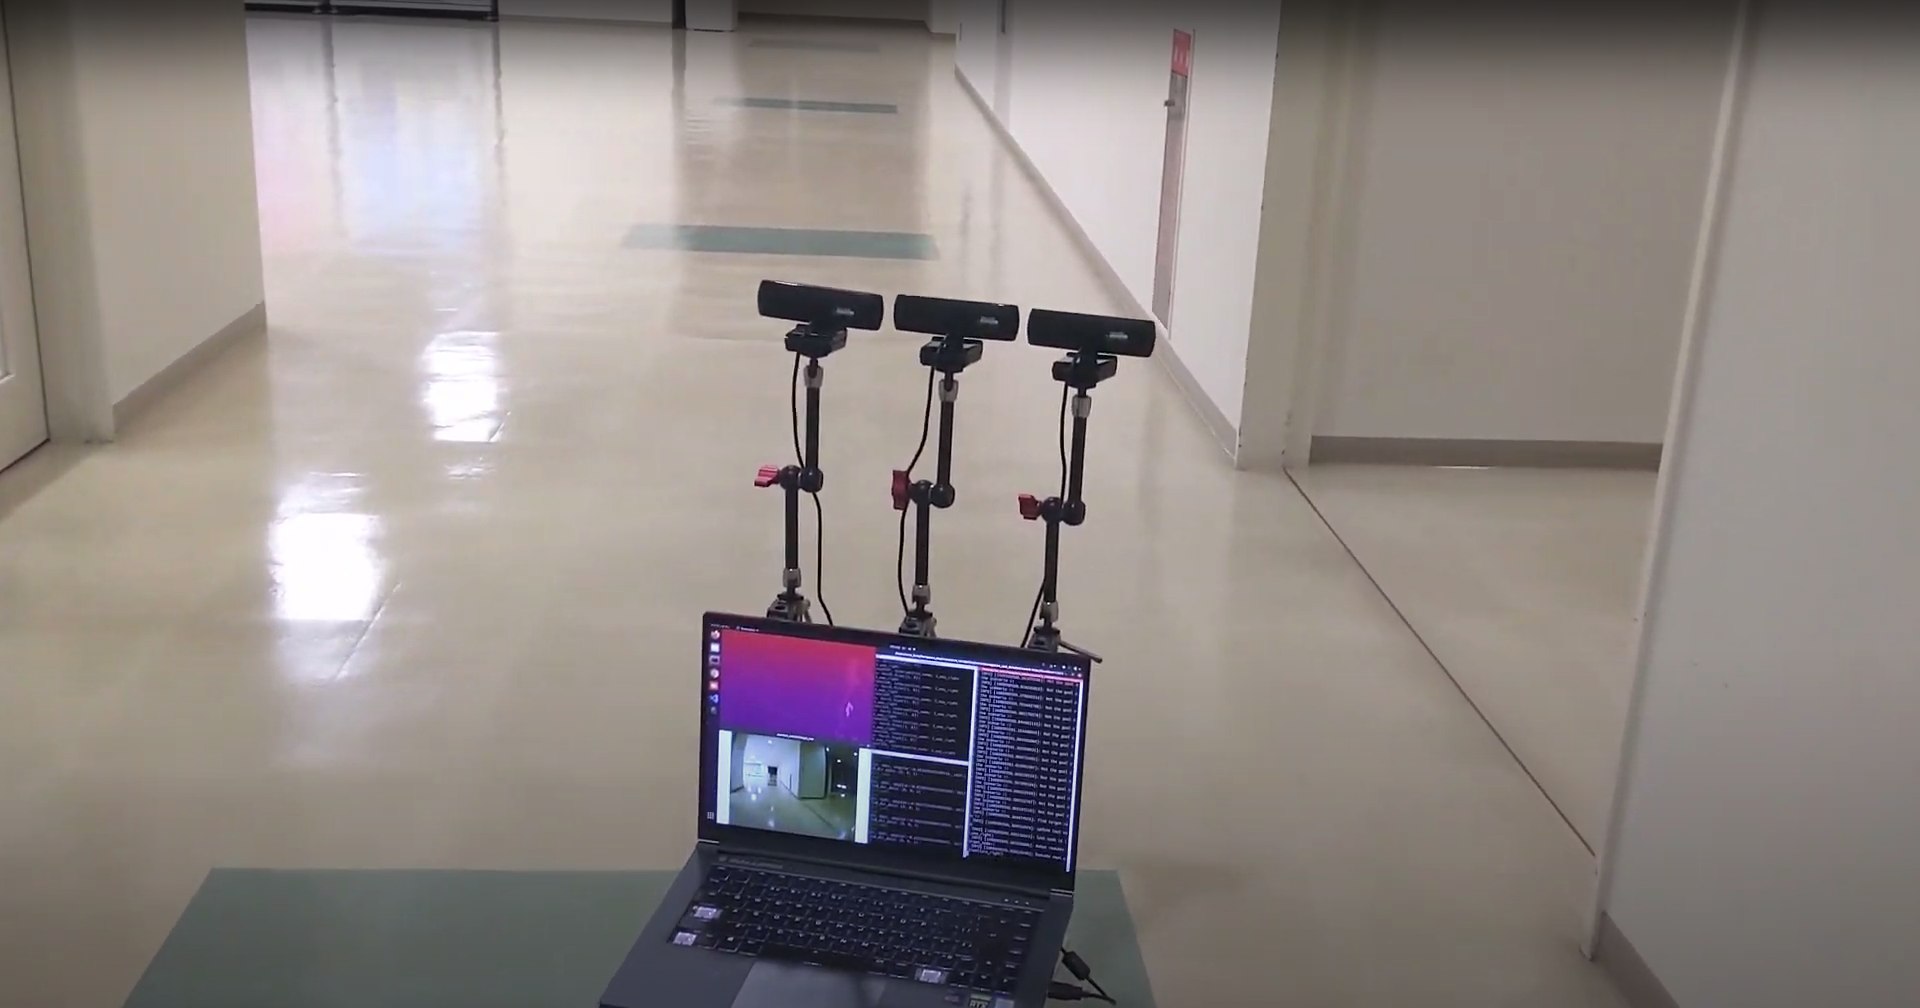
\includegraphics[keepaspectratio, width=80mm]{figs/exp_path_follow_2.png}
            \subcaption{右折(Third 3-way)}
            
        \end{minipage} &
        \begin{minipage}[t]{0.5\textwidth}
            \centering
            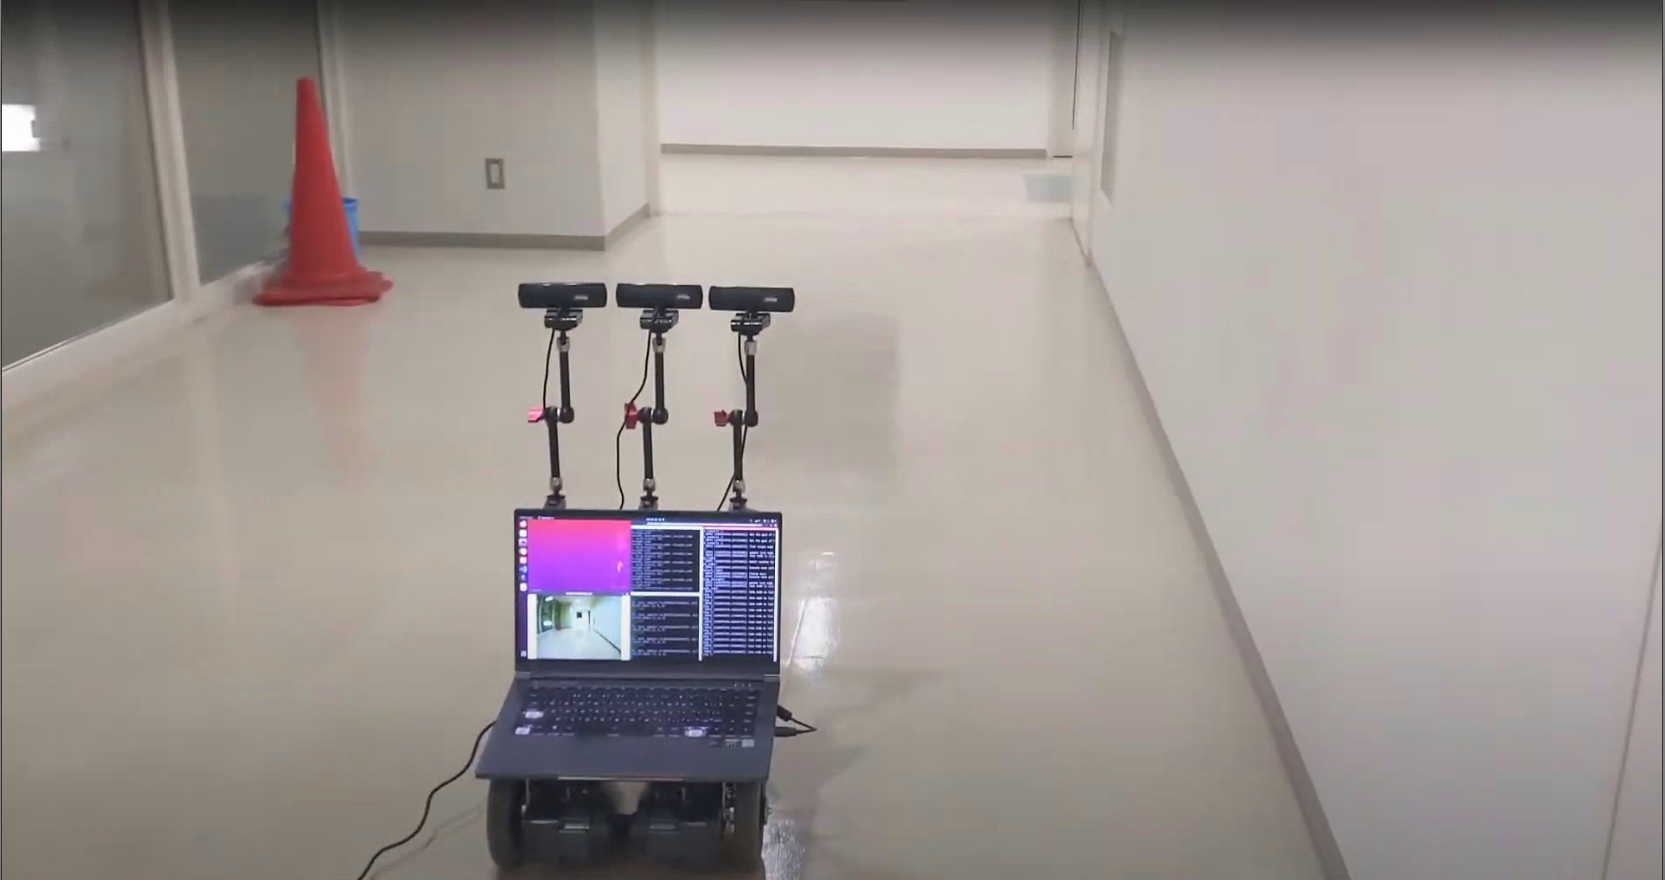
\includegraphics[keepaspectratio, width=80mm]{figs/exp_path_follow_4.png}
            \subcaption{突き当たりまで直進(straight road)}
        \end{minipage} \\
        \begin{minipage}[t]{0.5\textwidth}
            \centering
            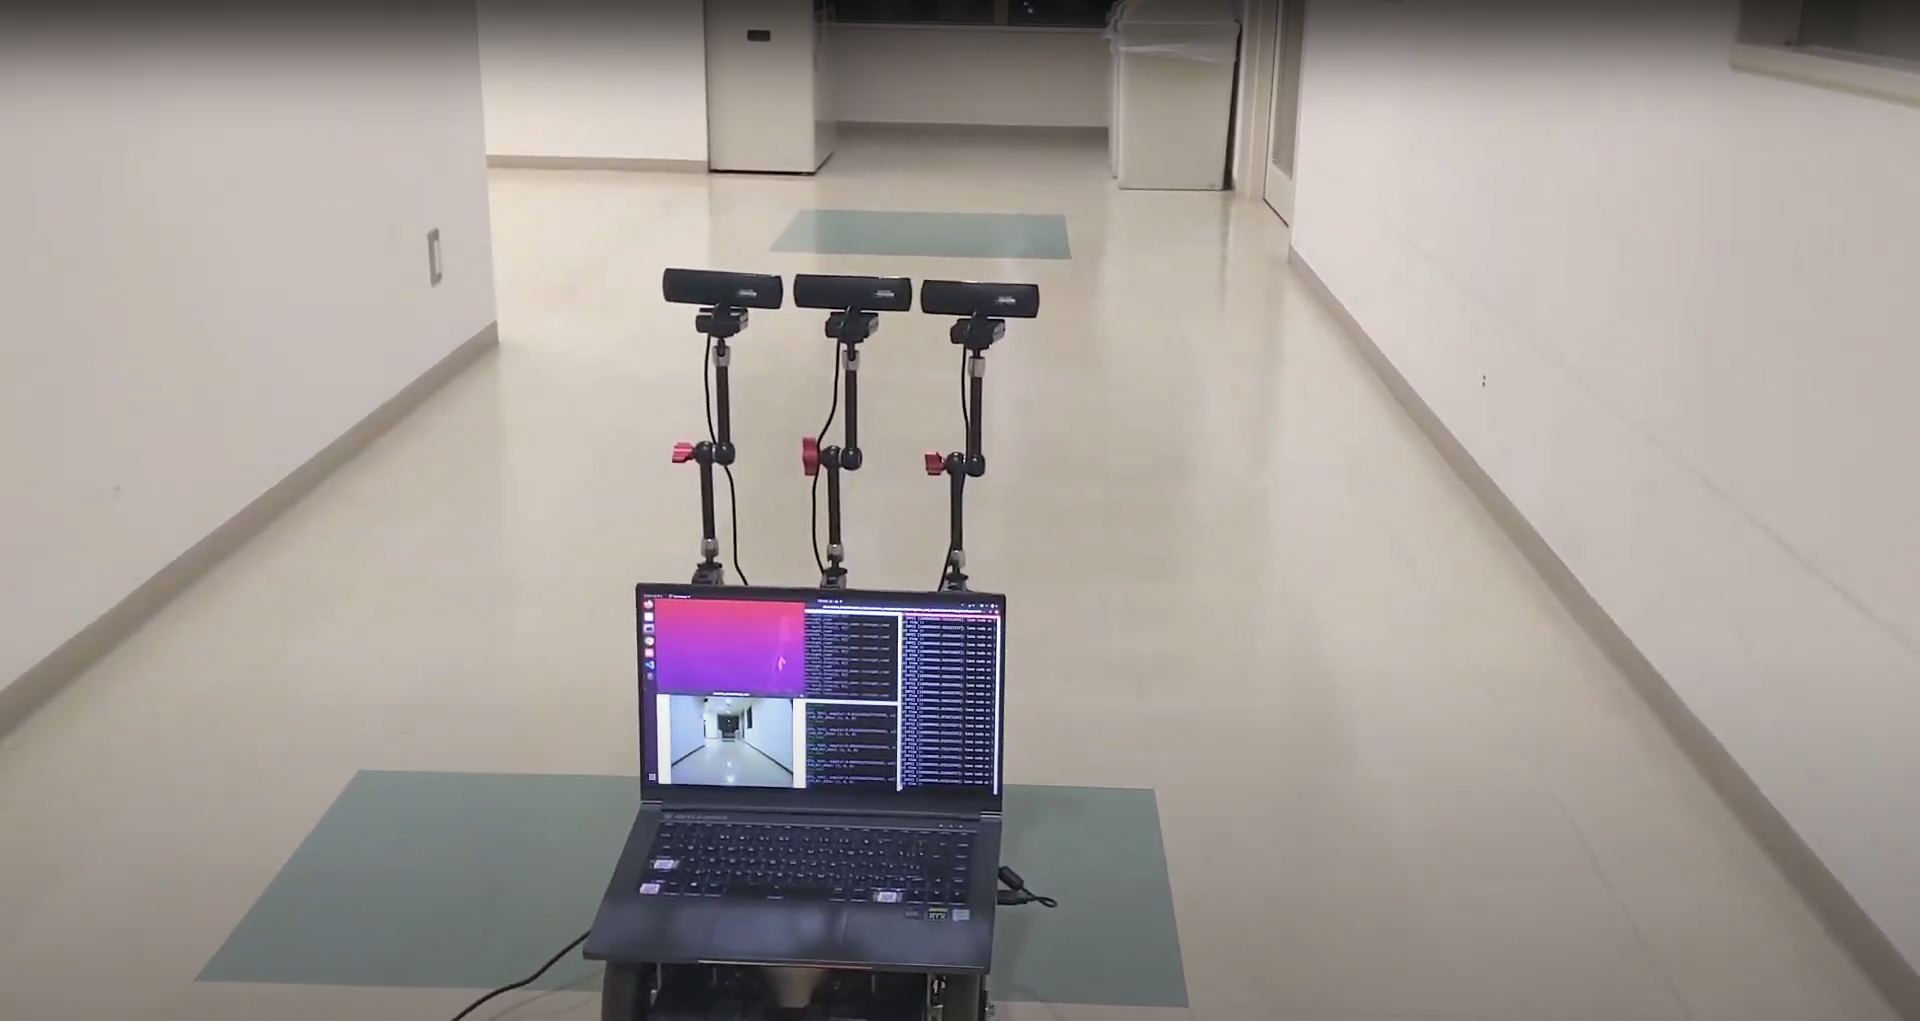
\includegraphics[keepaspectratio, width=80mm]{figs/exp_path_follow_5.png}
            \subcaption{左折(End)}
        \end{minipage}&
        \begin{minipage}[t]{0.5\textwidth}
            \centering
            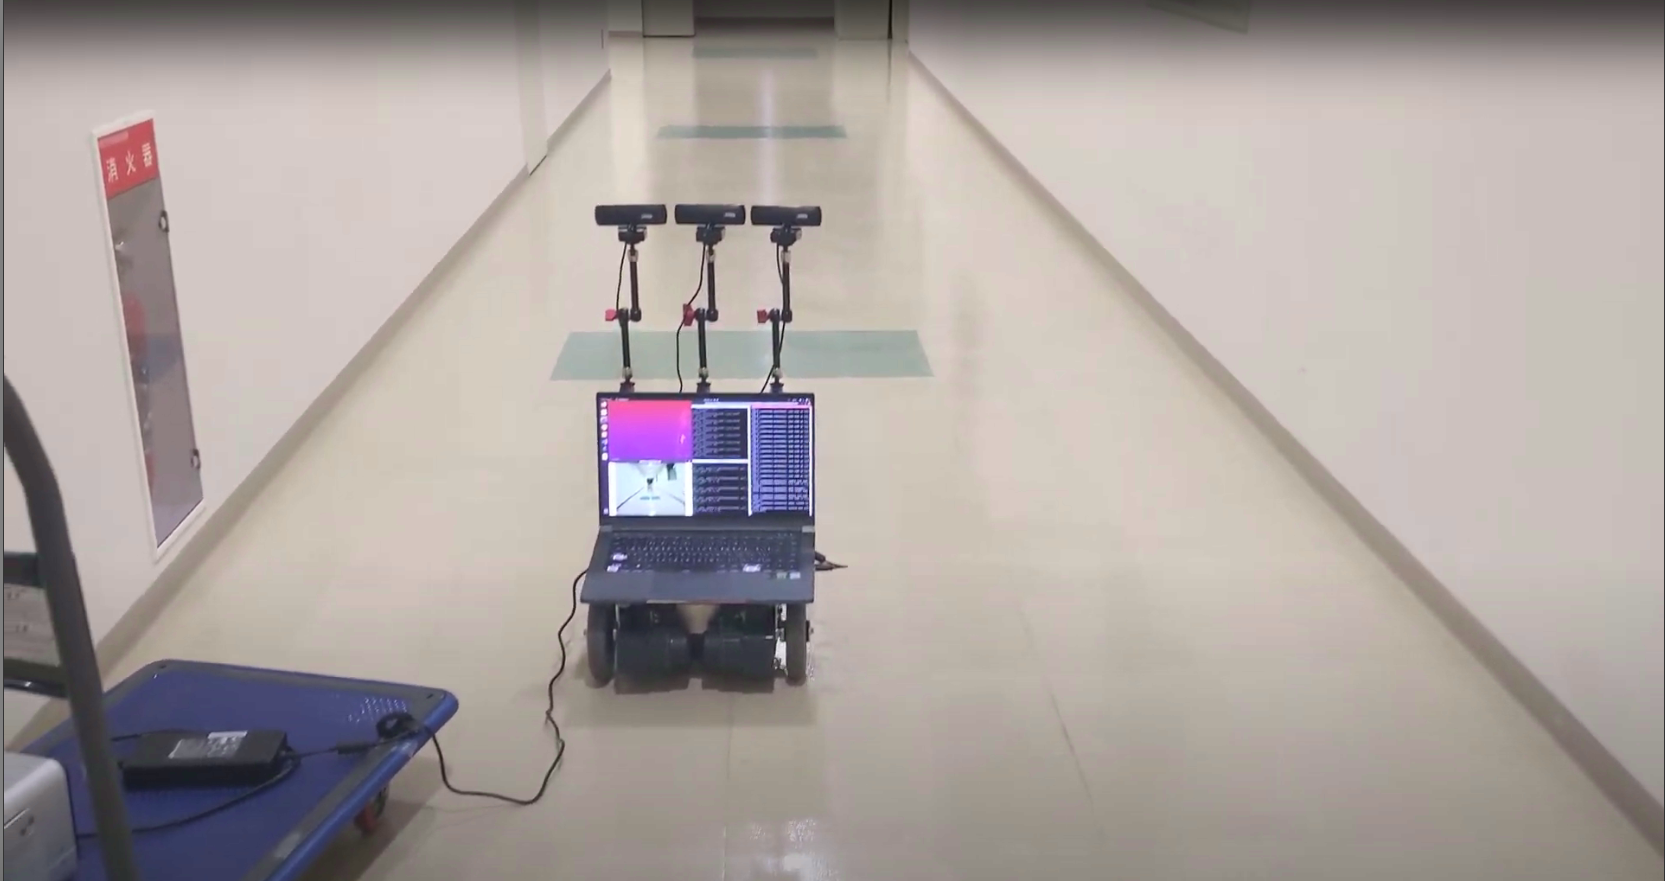
\includegraphics[keepaspectratio, width=80mm]{figs/exp_path_follow_6.png}
            \subcaption{突き当たりまで直進(straight road)}
        \end{minipage} \\
        \begin{minipage}[t]{0.5\textwidth}
            \centering
            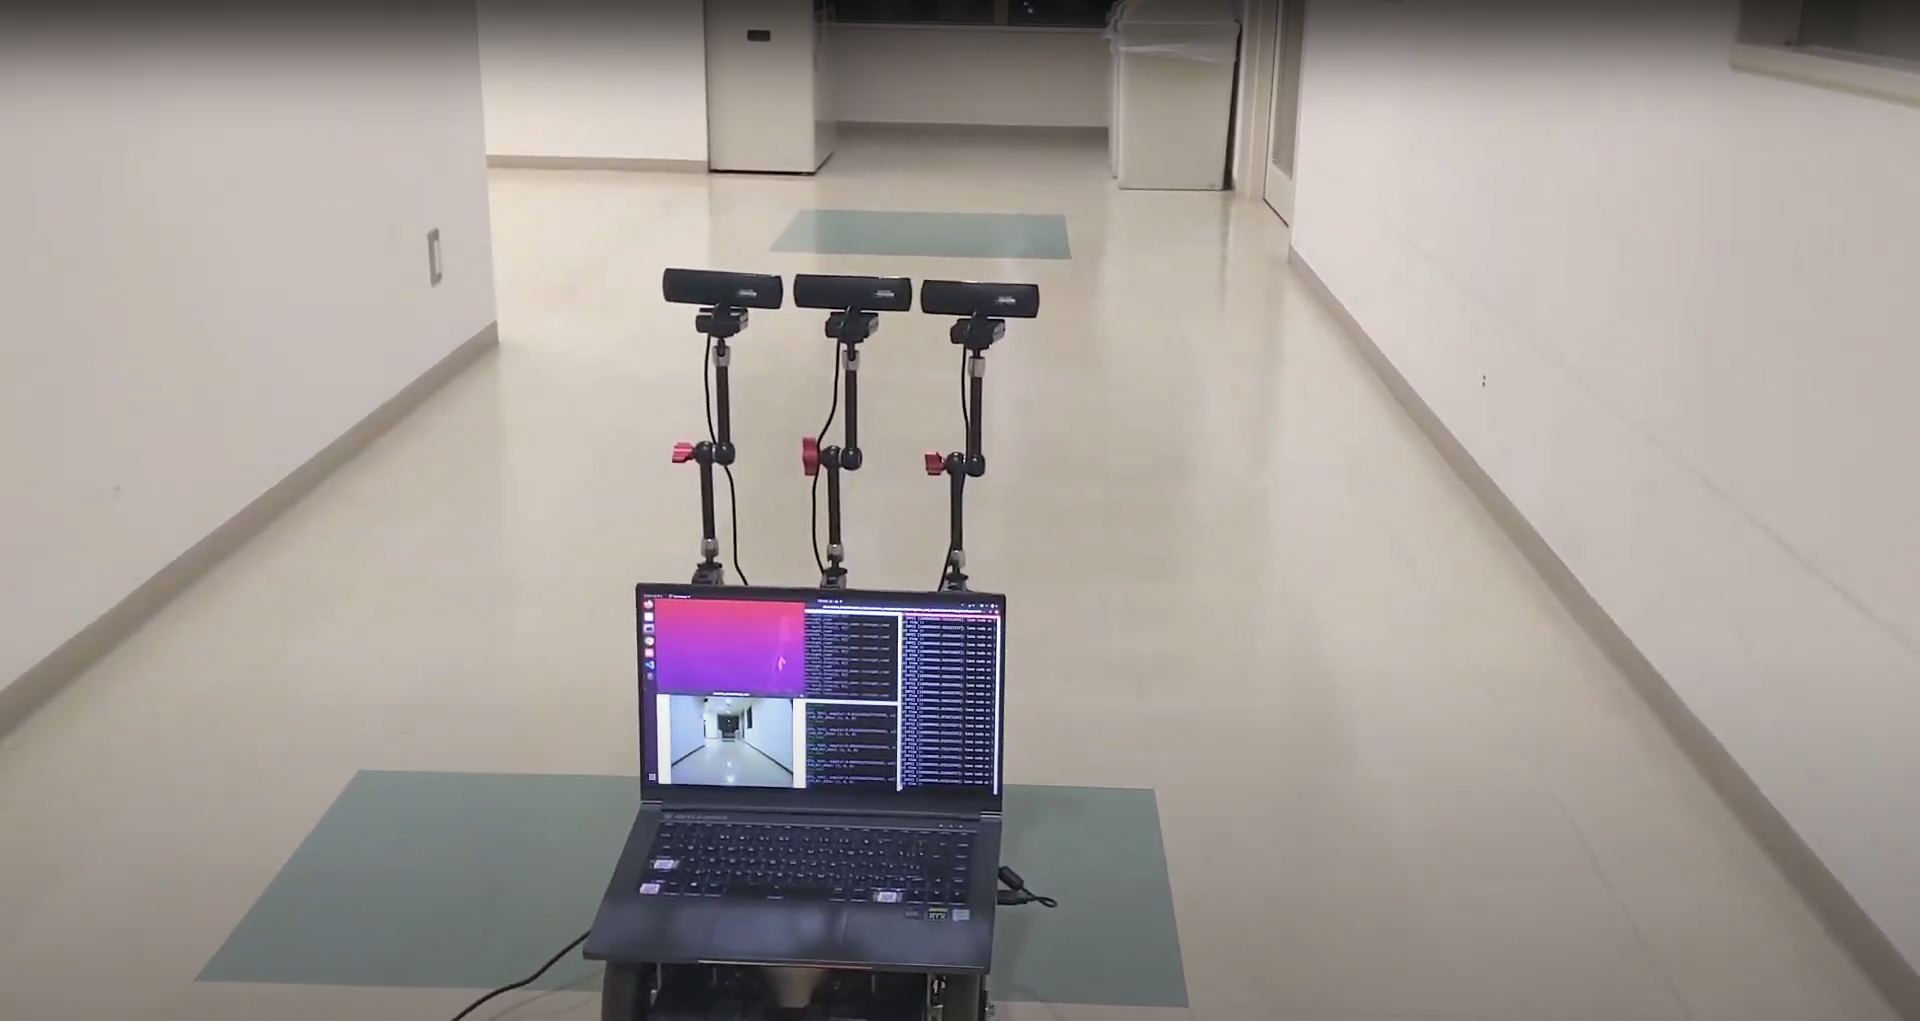
\includegraphics[keepaspectratio, width=80mm]{figs/exp_path_follow_7.png}
            \subcaption{停止(End)}
        \end{minipage}
    \end{tabular}

    \caption{Behavior of the robot applied the proposed method}\label{fig:exp_path}
\end{figure*}
% \begin{figure*}[htbp]\vspace*{-10zh}
%     \centering
%      \includegraphics[height=60mm,width=180mm]{./figs/exp_etc.png}
%      \caption{Behavior of path following in scenario24}\label{fig:exp}
% \end{figure*}
% \begin{table}[h!]
%     \centering
%     \caption{The number of assistances in the experiment}\label{tab:result}
%     % \begin{tabular}{ccclll}
        
%     % \begin{tabularx}{\textwidth}{X|X|X}
%     \begin{tabularx}{80mm}{|C|C|C|}
%     \hline
%     Scenario number used in the experiment & 
%     Number of assistances for deviating from the path & 
%     Number of assistances due to corridor classification failures \\
%     \hline
%     1       & 0         & 0             \\
%     5       & 0         & 0             \\
%     20      & 0         & 0             \\
%     21      & 0         & 0             \\
%     22      & 0         & 0             \\
%     24      & 0         & 0             \\
%     50      & 0         & 0             \\
%     \hline
%     % \end{tabular}
%     \end{tabularx}
%     \end{table}
\end{document}
